%----------------------------------------------------------------------------------------
%	CHAPTER - EVALUATION
%----------------------------------------------------------------------------------------

\chapter{Evaluation}

\label{ChapterEvaluation}

In the \textit{Evaluation} phase, the prototype is evaluated according to criteria from the \textit{Awareness of Problem} phase which either confirms or contradicts the initially defined hypothesis \citep{Vaishnavi2008}. The goal is to have an answer for the \gls{mrq}:
\begin{framed}
	\textit{\mrqtext}
\end{framed}

%----------------------------------------------------------------------------------------
%	SECTION 1
%----------------------------------------------------------------------------------------

\section{Introduction}

The evaluation of this prototype is based on the evaluation methods \textit{Testing} and \textit{Descriptive} as proposed by \cite{Hevner2004} and illustrated in Table \ref{tbl:designevaluationmethods} in Chapter \ref{EvaluationMethodology}. The \textit{Testing} evaluation method that focuses on the functional aspect in executing the artefact interfaces to find defects and failures as well as the structural aspect for metric evaluation have been part of the artefact development and therefore are already covered in Chapter \ref{ChapterDevelopment}. The \textit{Descriptive} evaluation methods are broken further down into several different \textit{Scenarios} which are discussed in the following chapters.


%----------------------------------------------------------------------------------------
%	SECTION 2
%----------------------------------------------------------------------------------------

\section{Descriptive Evaluation: Scenarios}

% Definition of the Scenarios
\newcommand{\scenone}{Checking for specific financial transaction}
\newcommand{\scentwo}{Comparing monthly expenses with previous yearsn}
\newcommand{\scenthree}{Figuring out why  account balance is zero in the middle of the month}
\newcommand{\scenfour}{Tracking the monthly expenses to not exceed the planned budget}

\citet[p.4]{Peffers2012} define the evaluation method of a prototype as: \blockquote{Implementation of an artifact aimed at demonstrating the utility or suitability of the artifact.} They continue that a prototype can help to demonstrate the efficiency of a design, and to show that it works as intended, is useful for its intended purpose, or at least has the potential to be at an expected level of performance \citep{Peffers2012}. For this, a set of detailed scenarios are defined that can demonstrate the utility of the prototype compared to the traditional way of executing the same tasks:
\begin{enumerate}[noitemsep,nolistsep]
	\item \scenone
	\item \scentwo
	\item \scenthree
	\item \scenfour
\end{enumerate}
Excluded from all scenarios are the steps required in order to log in to e-banking or to get an export of the data set for the prototype application. The starting point is either the entry page of e-banking or the just started prototype application. In order to measure the efficiency changes with the prototype, the following metrics are considered:
\begin{itemize}[noitemsep,nolistsep]
	\item Minimum number of steps to get to desired information
		\subitem Quantitative
	\item Exclusivity of presented data
		\subitem High = No other data is shown, only the requested one
		\subitem Medium = Some other data is shown, but clearly distinguishable
		\subitem Low = Much other data is shown, hard to find the right entry
	\item Comprehensibility
		\subitem High = Exact answer is directly presented
		\subitem Medium = Some interpretation is required to have an answer
		\subitem Low = Only meta data available; an answer has to be derived from it
\end{itemize}
While the first metric is of quantitative nature, the other two are qualitative and thus are split into three fuzzy values: High, Medium, Low. The exclusivity of the presented data is important in terms of whether only the required information is shown to the user and thus easy to identify, or if much more information is presented and the actually looked for part has to be searched for first. The comprehensibility focuses on how the data is presented and the difficulty to derive an exact answer to the question from it. \newline
At the current time, only the UBS e-banking offers an integrated way for categorizing financial transaction on such a detailed level. While other banking solutions also allow to check for specific executed payments (Scenario 1), they lack the capabilities to provide a detailed enough answers to the other scenarios. Due to this, the evaluation is conducted just with the UBS e-banking demo (\url{https://www.ubs.com/ebanking-demo-en}), but could be reproduced in future research with other banking solutions as well.


%-----------------------------------
%	SUBSECTION 1
%-----------------------------------
\subsection{Scenario 1}

\textbf{Scenario title:} \scenone

\textbf{Exemplary situation:} On Friday before the weekend, a bank transfer was create to pay an outstanding invoice. The user now would like to see if this payment has already been executed and the money transferred away from his account. 

While not exactly an exploratory scenario, it is a situation that can commonly happen and also question like these have to be answerable by the prototype whose since \gls{mdg} 4 defined that at least the same information as existing applications must be provided.

%-----------------------------------
%	SUBSUBSECTION 1
%-----------------------------------

\subsubsection{E-Banking}

With the e-banking demo of UBS, the information can be found by navigating over two screens, which depending on the amount of transaction can require 2 - 10 mouse clicks to reach the final screen. After navigating to the "Expenses" view, all transactions of the last 30 days are shown by default, giving the user the option to apply a more specific filter or look for the transaction on this bigger list. The visualized flow for this scenario is shown in Figure \ref{fig:scenariooneebanking}.
\begin{enumerate}[noitemsep,nolistsep]
	\item Go via "Budget" to "Expenses" (2 clicks)
	\item OPTIONAL: Set filter for specific date range (4 clicks)
	\item OPTIONAL: Set filter for amount range (4 clicks)
	\item OPTIONAL: Scroll down the list of transactions if there are too many
	\item Find the transaction in the list, or not
\end{enumerate}
\begin{figure}[h]
	\begin{center}
		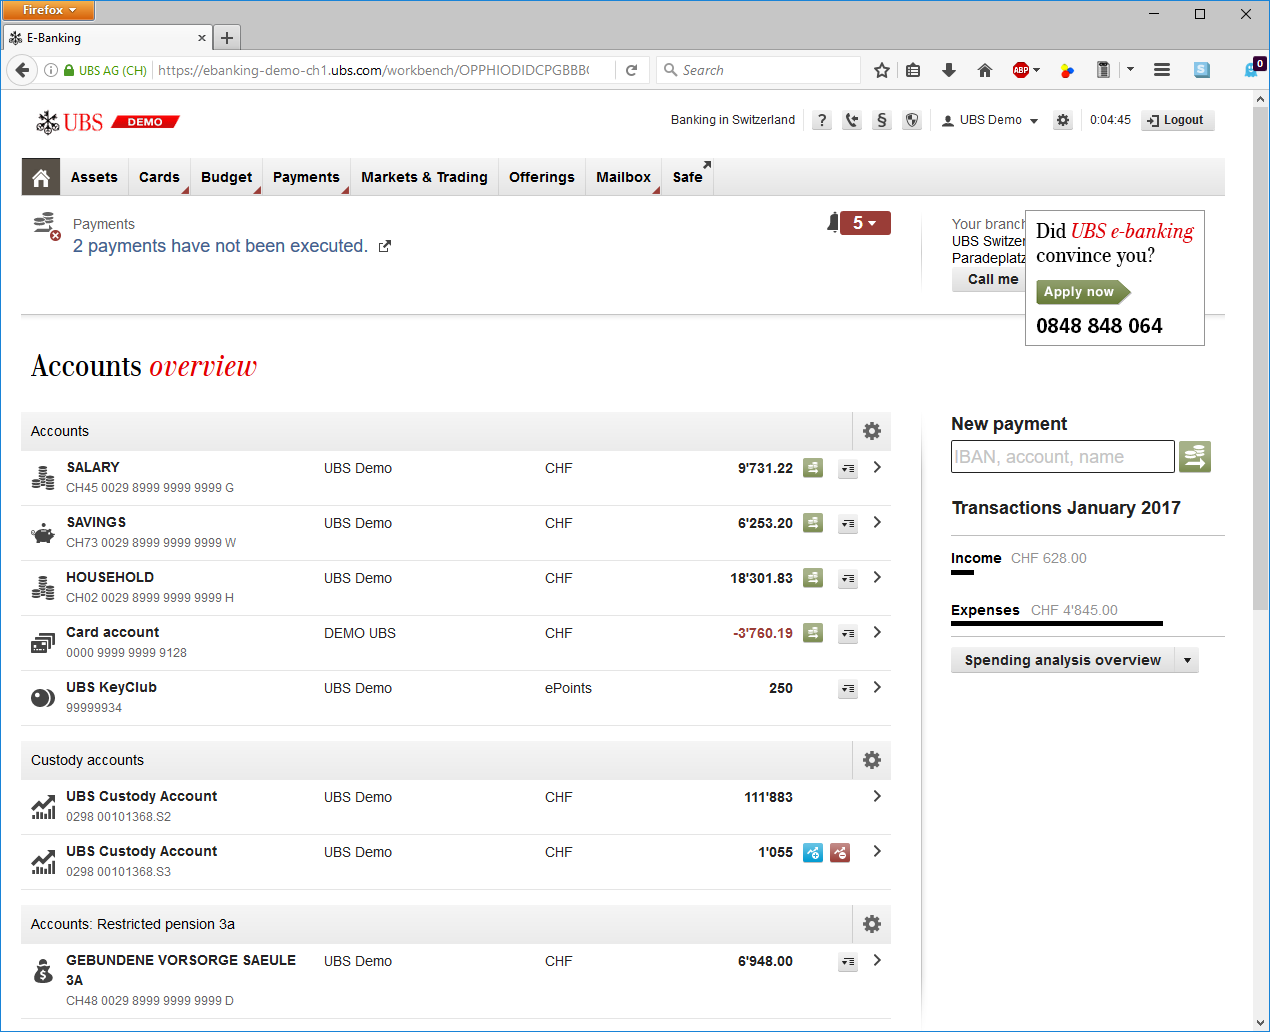
\includegraphics[width=4.7cm]{03_Figures/09_Evaluation/UBS_1_Overview.png}
		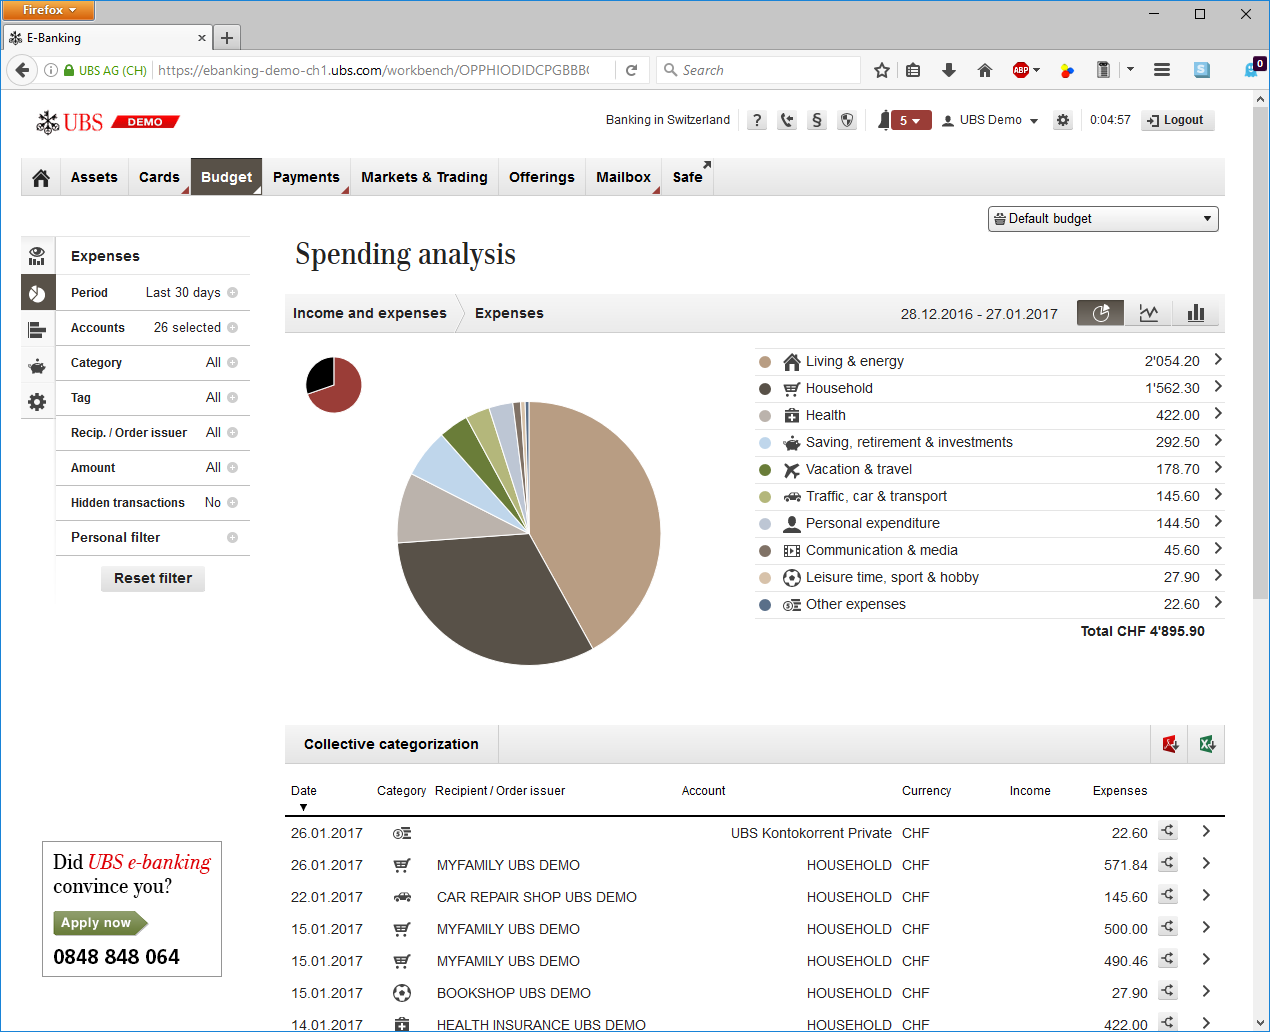
\includegraphics[width=4.7cm]{03_Figures/09_Evaluation/UBS_2_SpendingAnalysis.png}
		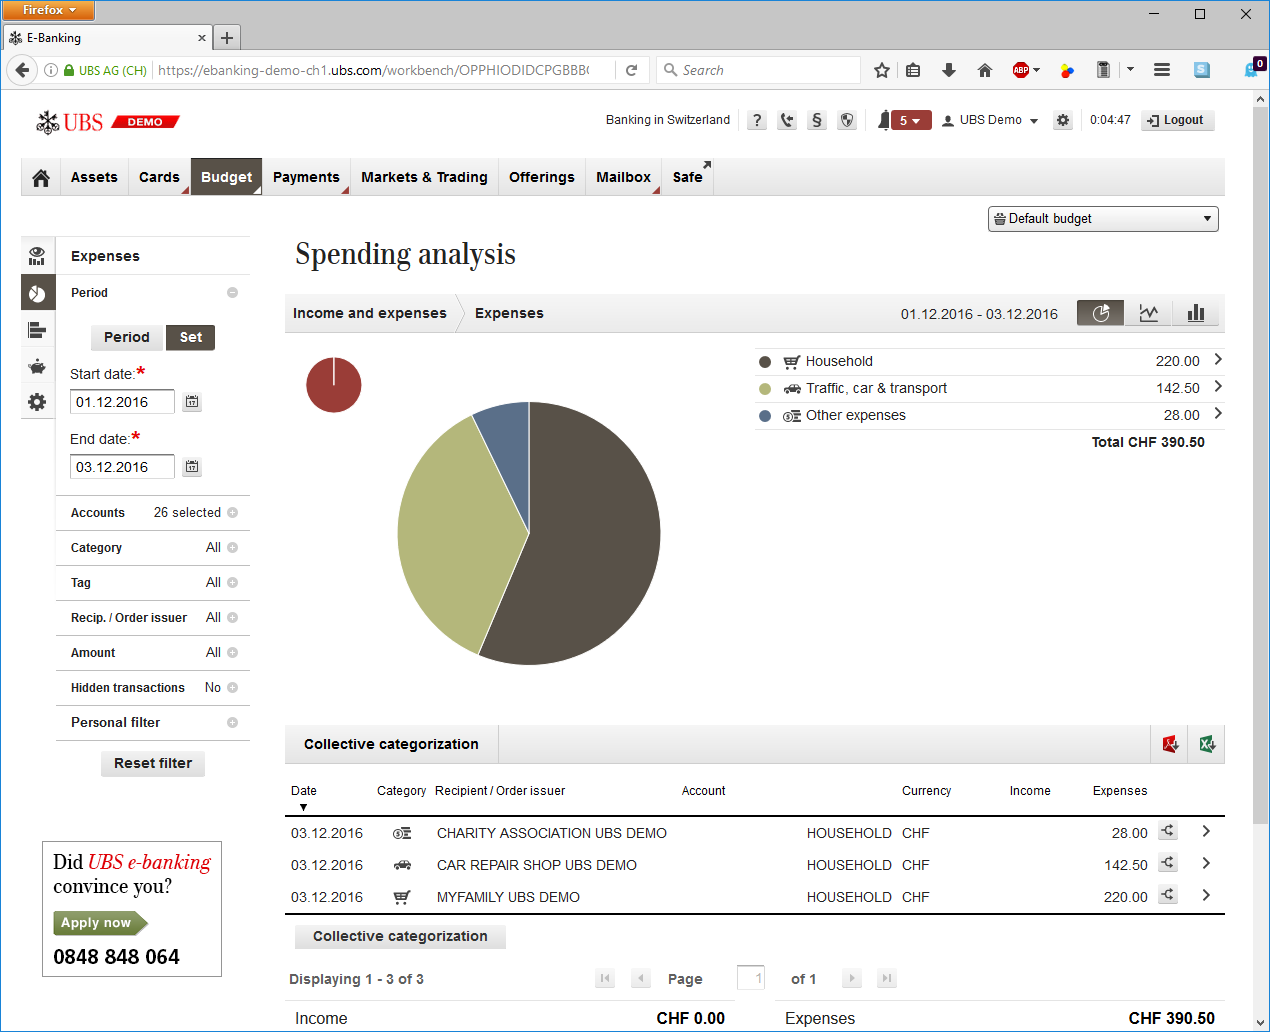
\includegraphics[width=4.7cm]{03_Figures/09_Evaluation/UBS_2_SpendingAnalysis_Filter.png}
		\caption{Visualized flow of screens in e-banking demo for Scenario 1}
		\label{fig:scenariooneebanking}
	\end{center}
\end{figure}


\textbf{Evaluation:} Due to displaying all transaction of the last 30 days by default, the initial exclusivity of the data is relatively low. If additional filters are applied, the exclusivity can vary between medium and high, depending on how specific it is set. The narrower it is, the more mouse clicks are required. In terms of the comprehensibility of the data, some interpretation is required in order to know whether the transaction did not execute, or if it just has been filtered out.
\begin{itemize}[noitemsep,nolistsep]
	\item Min. number of steps: \textbf{2 - 10}
	\item Exclusivity: \textbf{High} (+2 filters), \textbf{Medium} (+1 filter), \textbf{Low} (default filter)
	\item Comprehensibility: \textbf{Medium}
\end{itemize}


%-----------------------------------
%	SUBSUBSECTION 2
%-----------------------------------

\subsubsection{Prototype Application}

With the prototype application, the answer to this scenario can be found in 3-5 interaction steps, depending on the amount of transactions. The visualized flow for this scenario is shown in Figure \ref{fig:scenariooneprototype}.
\begin{enumerate}[noitemsep,nolistsep]
	\item Activate corresponding category, OR activate all (View 4)
	\item Click on the current month in the Year Overview bar chart (View 1)
	\item OPTIONAL: Click on the specific day in the Month Overview bar chart (View 2)
	\item OPTIONAL: Scroll down the list of transactions if there are too many (View 5)
	\item Find the transaction in the list, or not (View 5)
\end{enumerate}
\begin{figure}[h]
	\begin{center}
		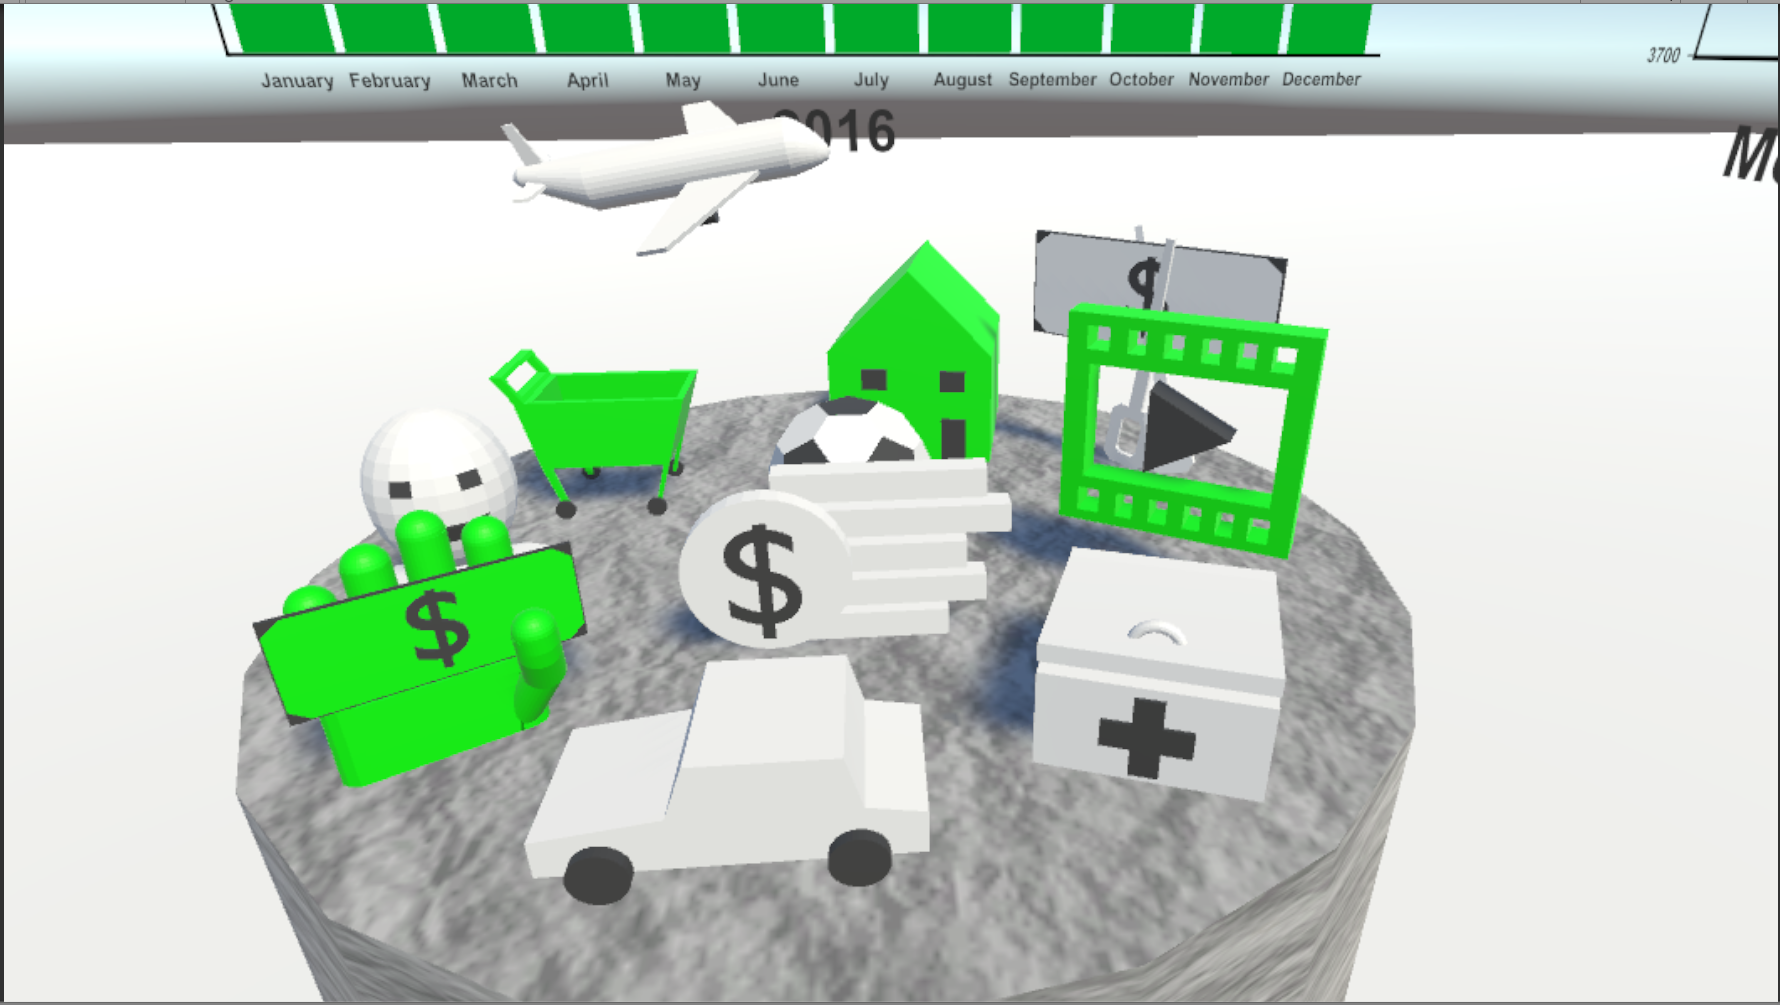
\includegraphics[width=2.8cm]{03_Figures/08_Development/View4_CategoriesFiltering.png}
		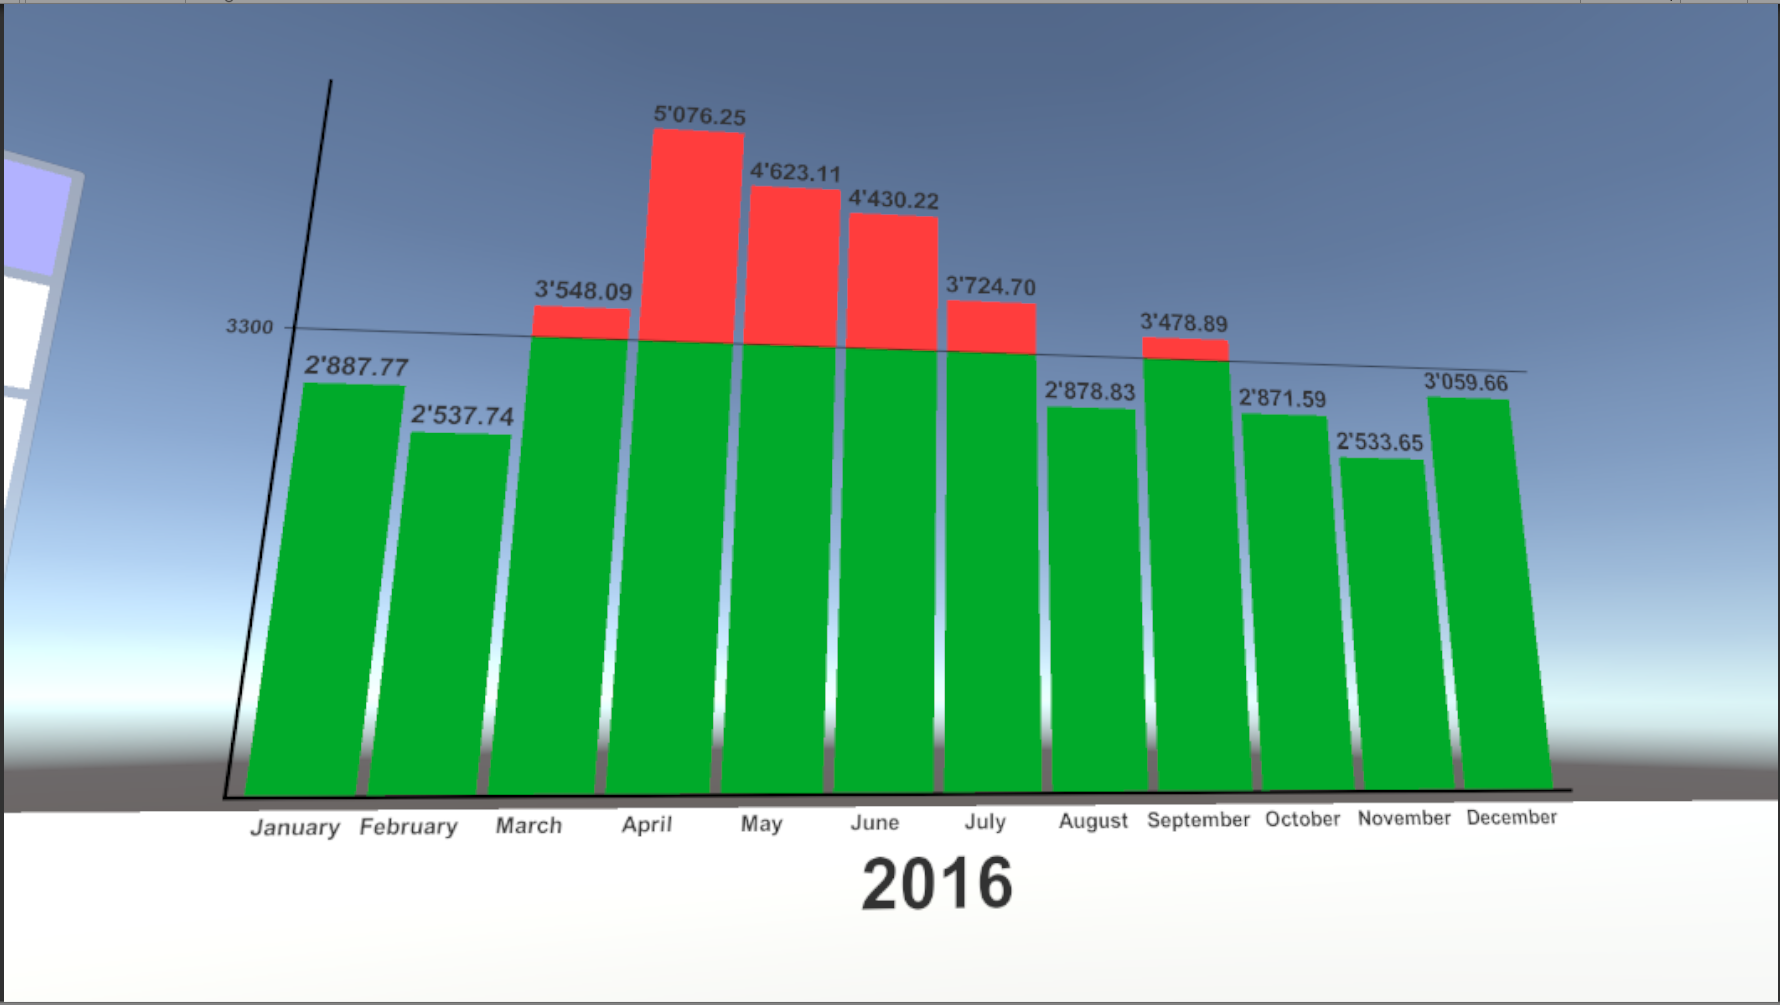
\includegraphics[width=2.8cm]{03_Figures/08_Development/View1_YearOverview.png}
		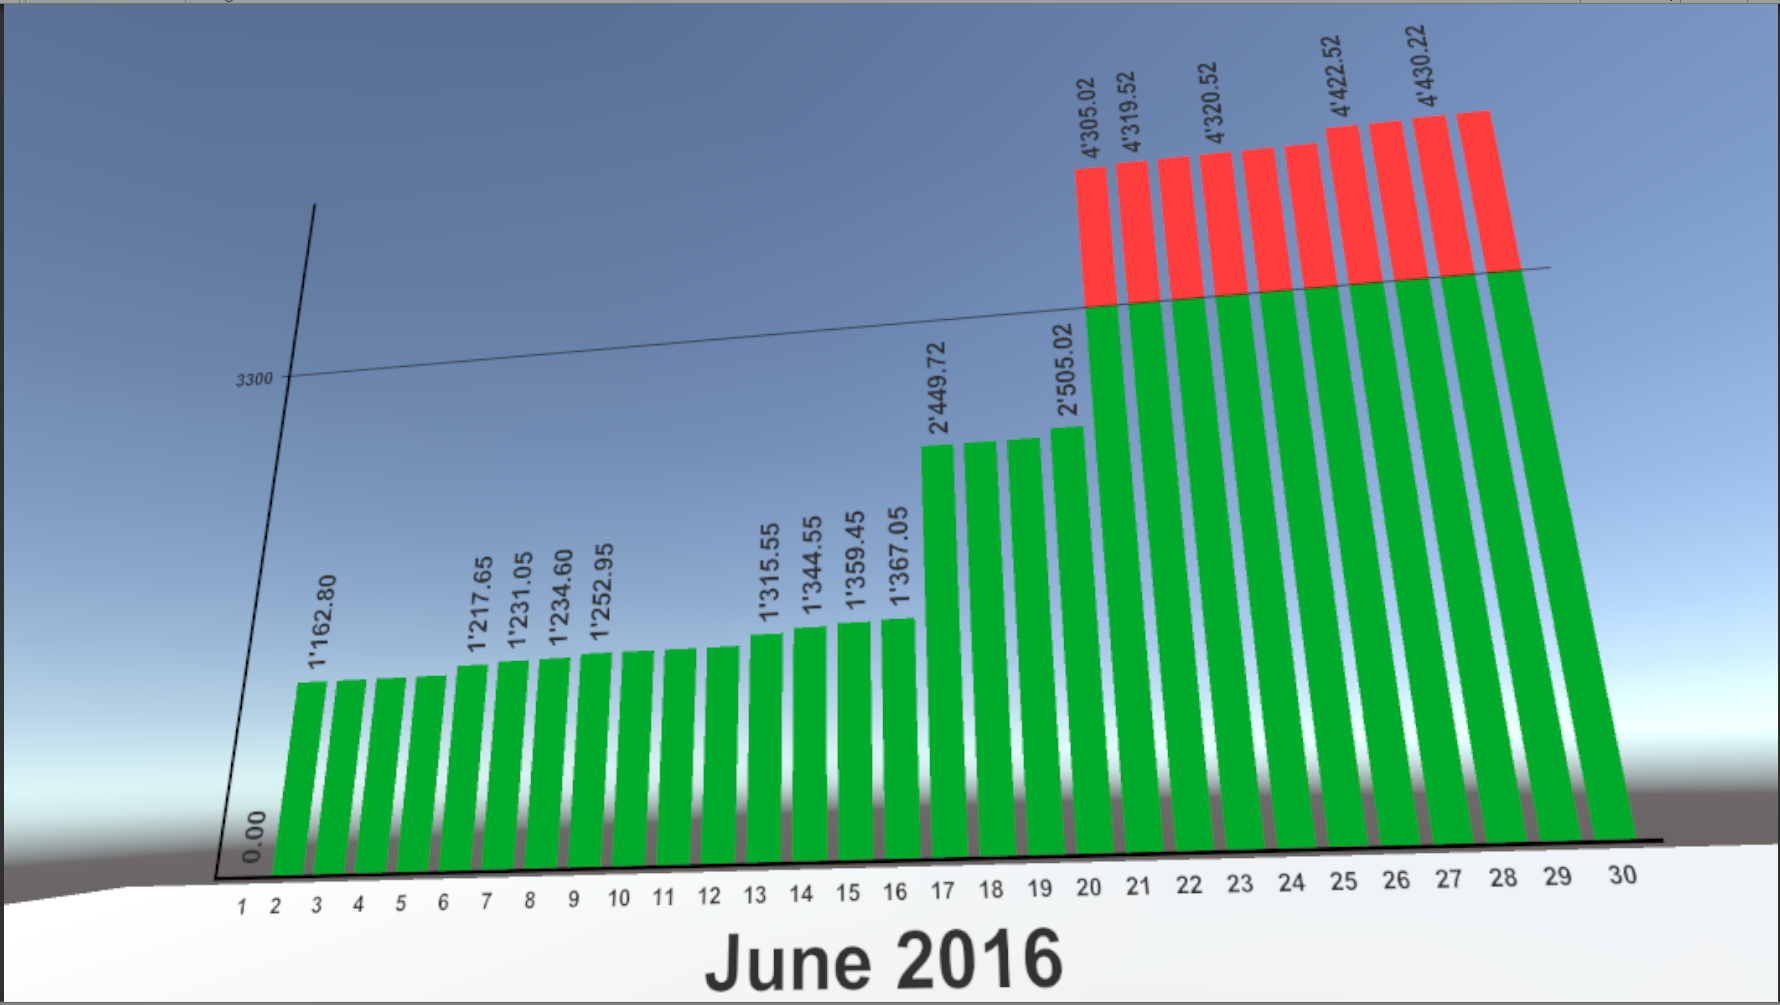
\includegraphics[width=2.8cm]{03_Figures/08_Development/View2_MonthOverview.png}
		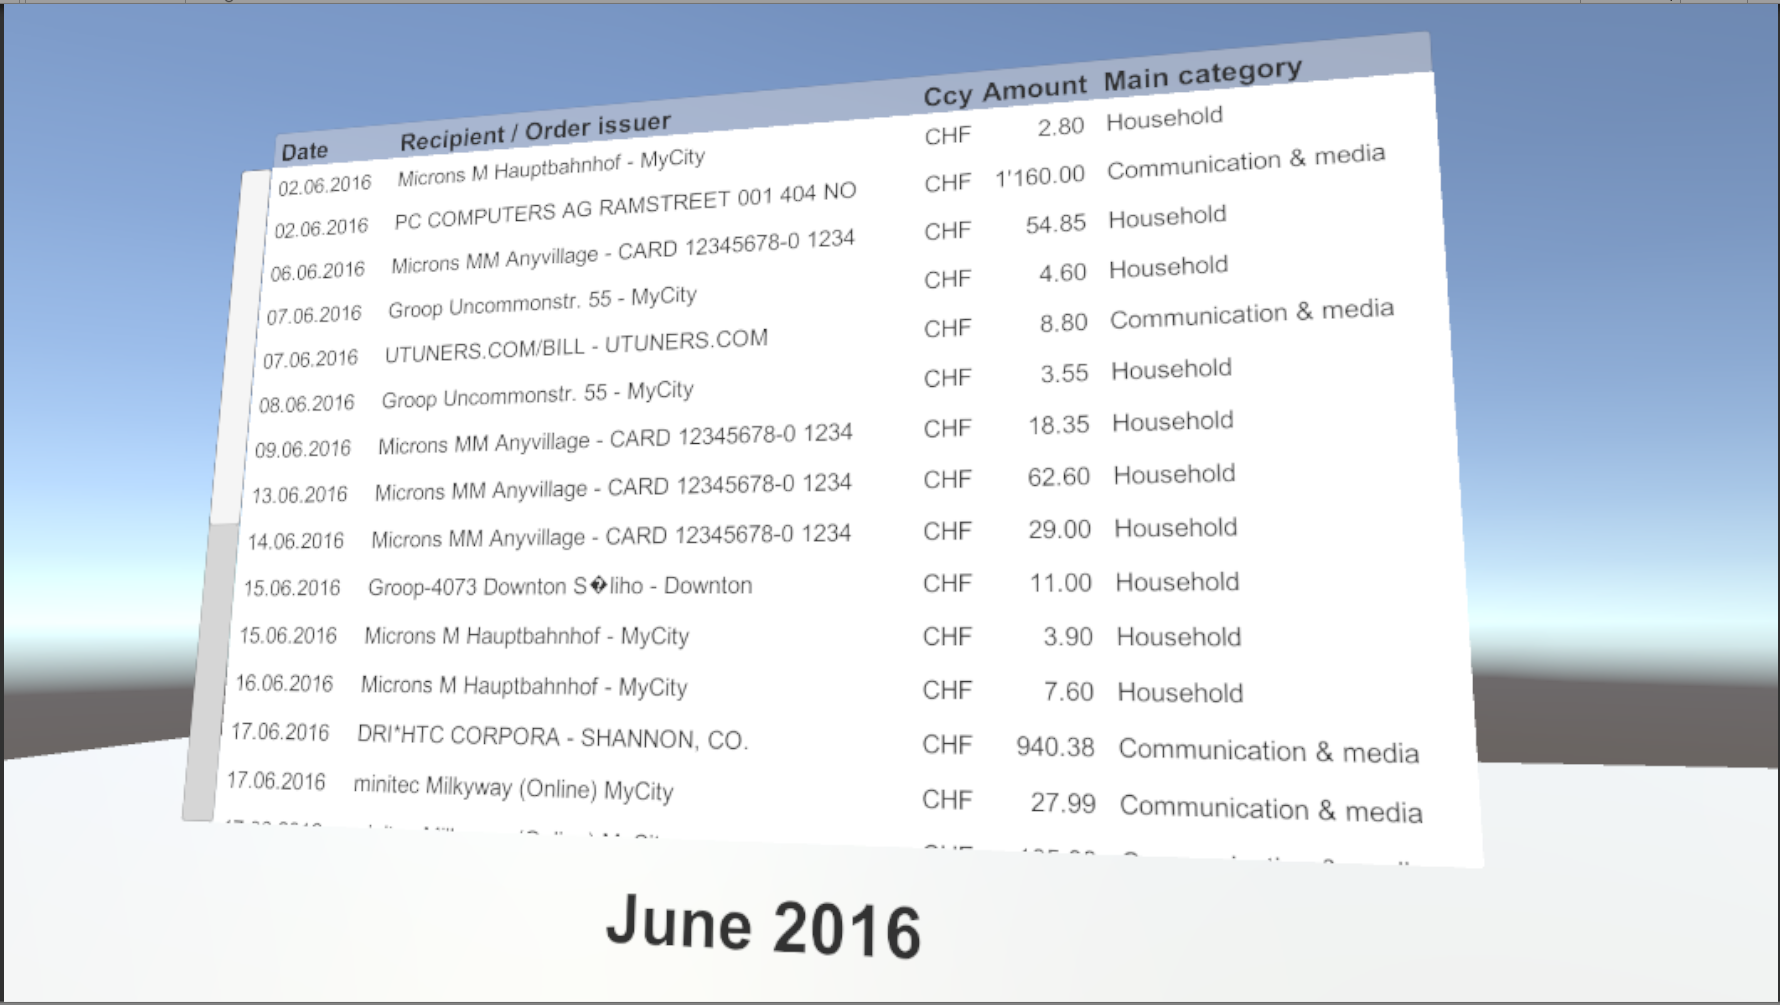
\includegraphics[width=2.8cm]{03_Figures/08_Development/View5_FinTransactionsOverview.png}
		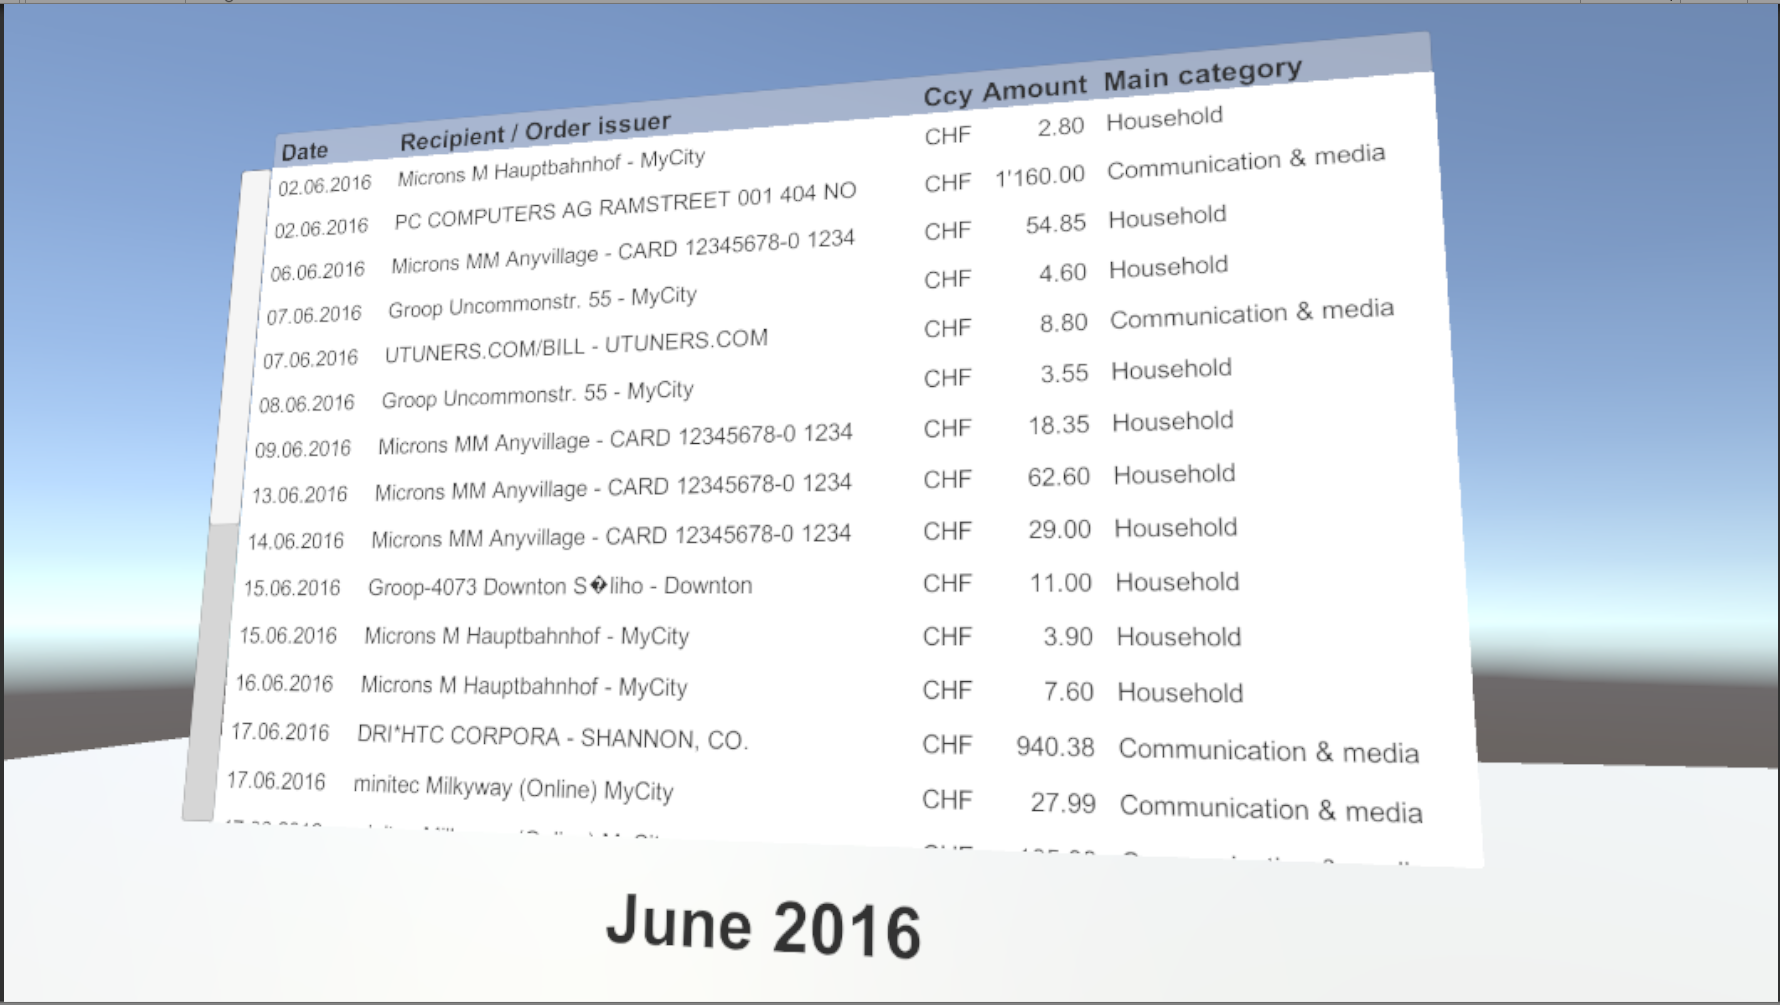
\includegraphics[width=2.8cm]{03_Figures/08_Development/View5_FinTransactionsOverview.png}
		\caption{Visualized flow of views in prototype for Scenario 1}
		\label{fig:scenariooneprototype}
	\end{center}
\end{figure}


\textbf{Evaluation:} Depending on the amount of rows in the table, the exclusivity can be rated a bit higher or not. Selecting a specific day in the Month Overview clearly helps to reduce the amount of rows, but might require additional interaction steps if it is not known on what exact date the transaction was executed. Since it is not directly possible to search for a specific booking text or similar, some interpretation on the table rows is required.
\begin{itemize}[noitemsep,nolistsep]
	\item Min. number of steps: \textbf{3 - 5}
	\item Exclusivity: \textbf{Medium} (with filtered day), \textbf{Low} (without)
	\item Comprehensibility: \textbf{Medium}
\end{itemize}


%-----------------------------------
%	SUBSUBSECTION 1
%-----------------------------------

\subsubsection{Conclusion: Scenario 1}

Table \ref{tbl:scenarioonecomparison} summarizes the individual evaluations of the prototype and the e-banking regarding the first scenario. It can be seen that has only half of the maximum required amount of steps compared to e-banking, but regarding the exclusivity cannot compete as the filter criteria are much more limited and thus also display more unwanted data. The comprehensibility is for both the same, as the format of the displayed data is equivalent.
\begin{table}[h]
	\begin{center}
		\begin{tabular}{ | p{3.2cm} | p{3.8cm} | p{3.5cm} | p{2.5cm} | }
			\hline
			\textbf{Metric} & \textbf{E-Banking} & \textbf{Prototype} & \textbf{Winner} \\
			\hline
				Min. no. of steps: & 2 - 10 & 3 - 5 & Prototype \\
			\hline
				Exclusivity: & Low / Medium / High & Low / Medium & E-Banking \\
			\hline
				Comprehensibility: & Medium & Medium & Draw \\
			\hline
		\end{tabular}
		\caption{Scenario 1: Comparison of prototype and e-banking}
		\label{tbl:scenarioonecomparison}
	\end{center}
\end{table}


%-----------------------------------
%	SUBSECTION 2
%-----------------------------------

\subsection{Scenario 2}

\textbf{Scenario title:} \scentwo

\textbf{Exemplary situation:} Since their first child was born, a family is wondering how their household and travelling expenses have changed compared to previous years.


%-----------------------------------
%	SUBSUBSECTION 1
%-----------------------------------

\subsubsection{E-Banking}

Compared to Scenario 1, many more filters need to be applied for this second scenario which results in an increased amount of interaction steps to a total of 14 mouse clicks, on the same two screens as before. Since the option to toggle the individual categories are hidden behind an expandable section, an additional click is required. The same applies to the situation when the view is shifted to the previous years when again both start and end date need to be manually adjusted. The visualized flow for this scenario is shown in Figure \ref{fig:scenariotwoebanking}.
\begin{enumerate}[noitemsep,nolistsep]
	\item Go via "Budget" to "Expenses" (2 clicks)
	\item Set filter for the two categories (4 clicks)
	\item Set filter for specific date range in current year (4 clicks)
	\item Set filter for specific date range in previous year (4 clicks)
\end{enumerate}
\begin{figure}[h]
	\begin{center}
		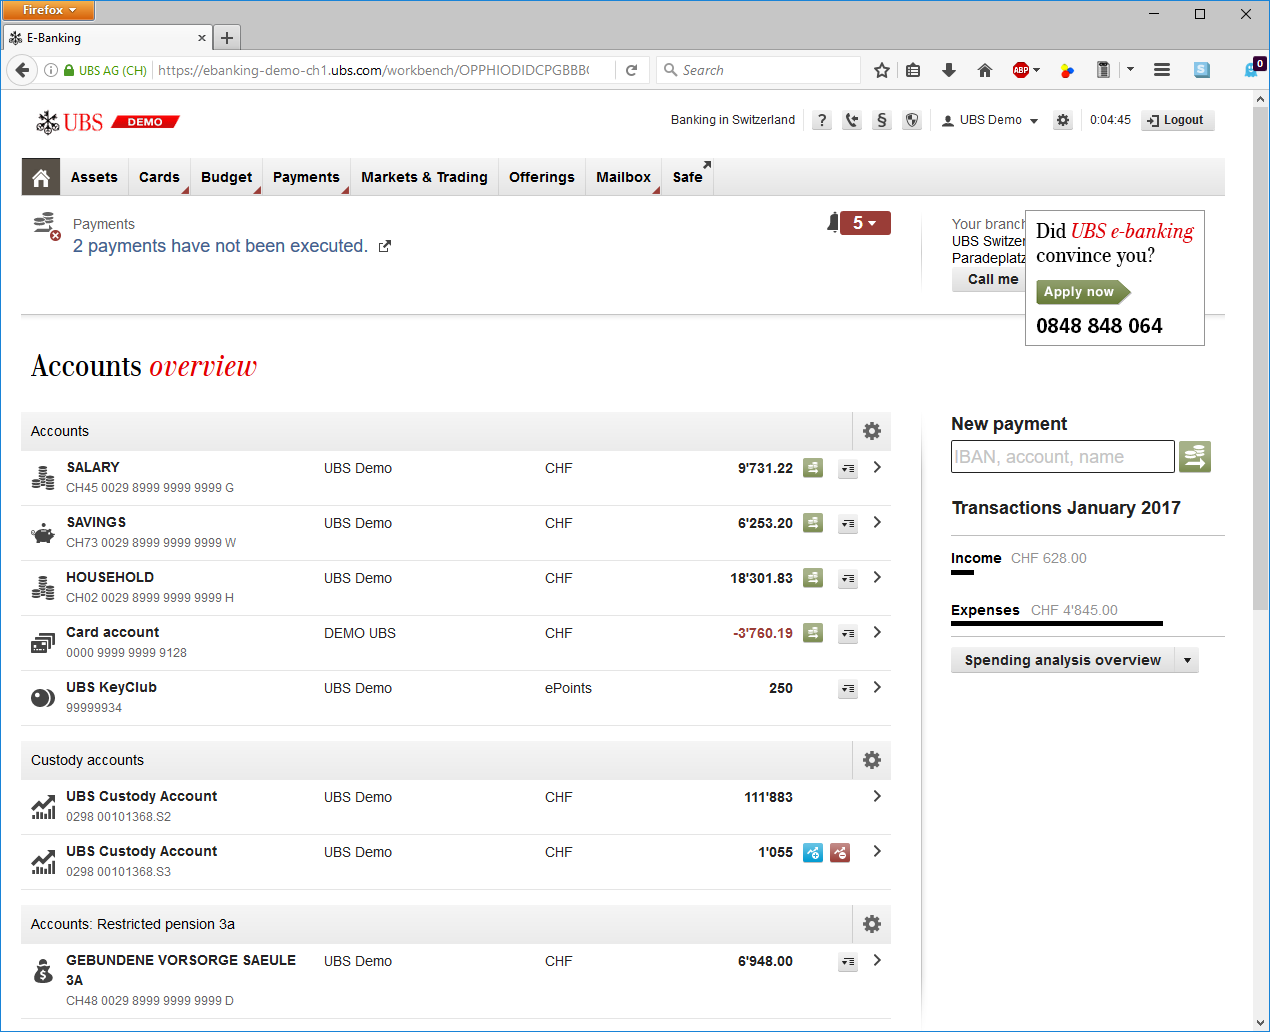
\includegraphics[width=2.8cm]{03_Figures/09_Evaluation/UBS_1_Overview.png}
		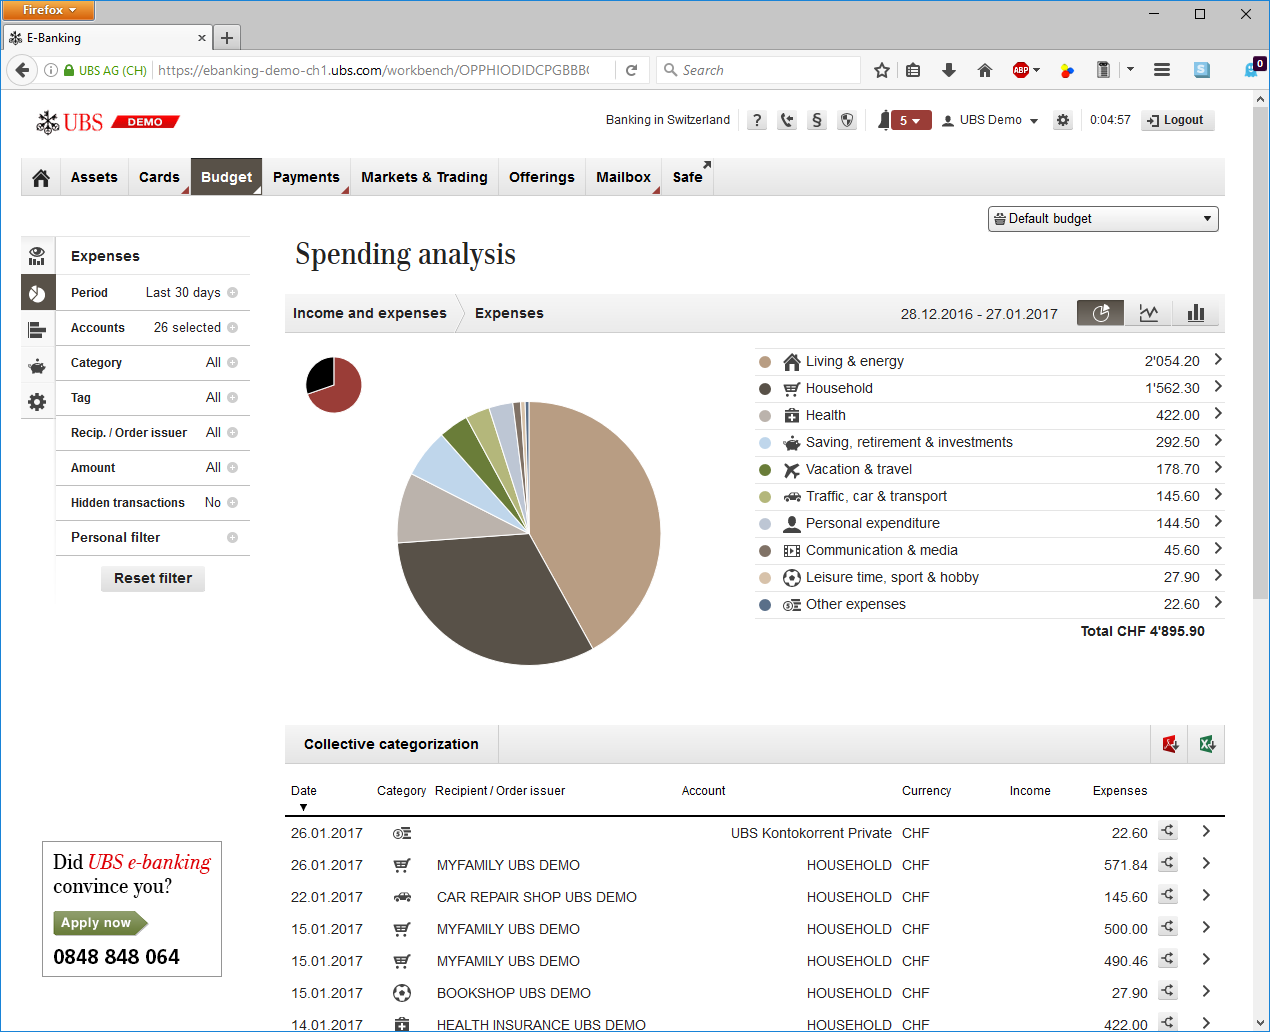
\includegraphics[width=2.8cm]{03_Figures/09_Evaluation/UBS_2_SpendingAnalysis.png}
		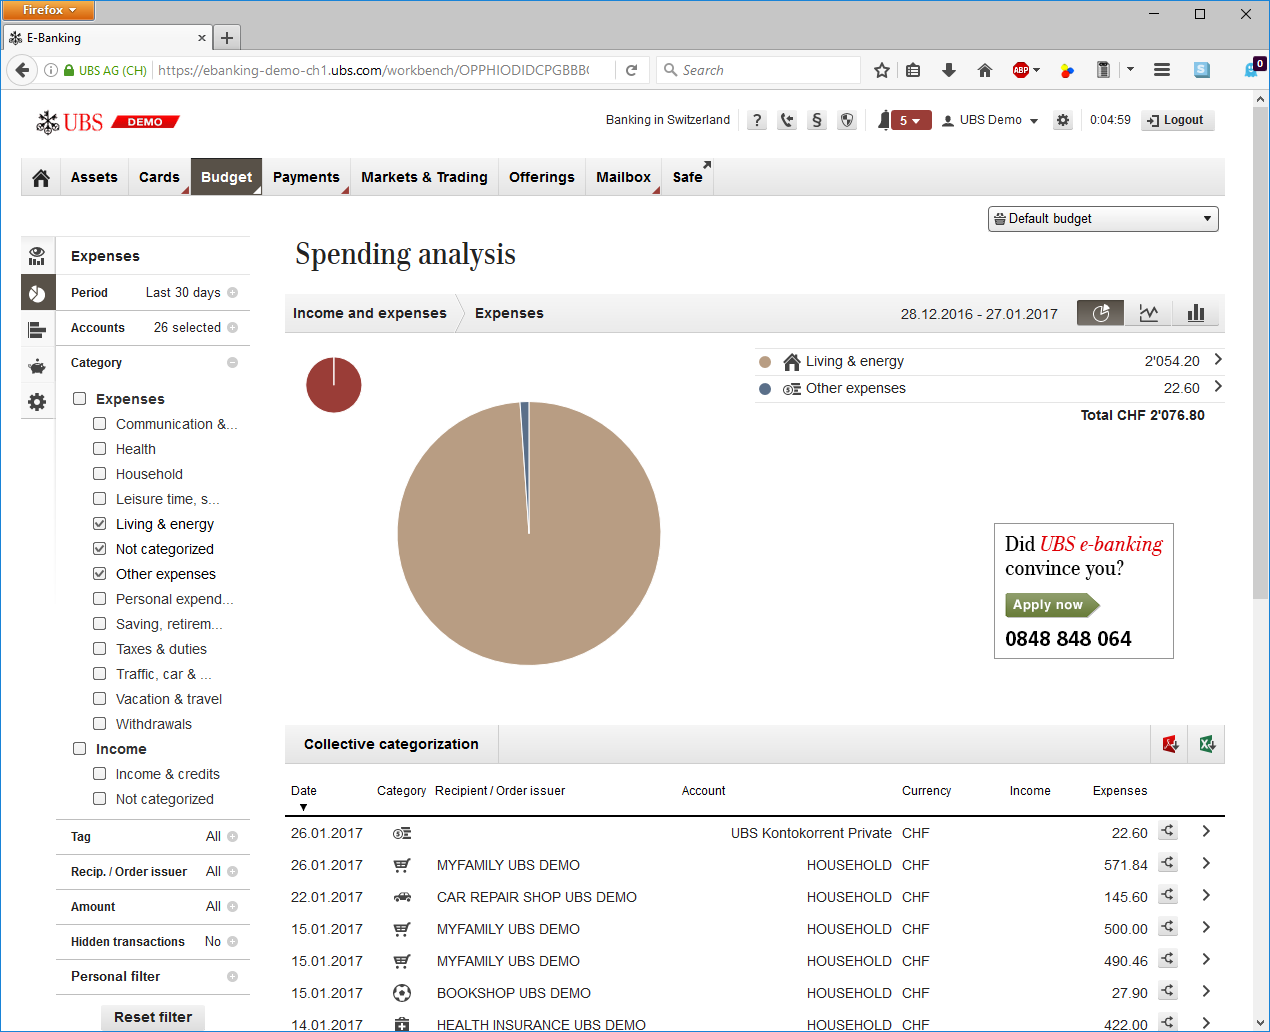
\includegraphics[width=2.8cm]{03_Figures/09_Evaluation/UBS_2_SpendingAnalysis_FilterCat.png}
		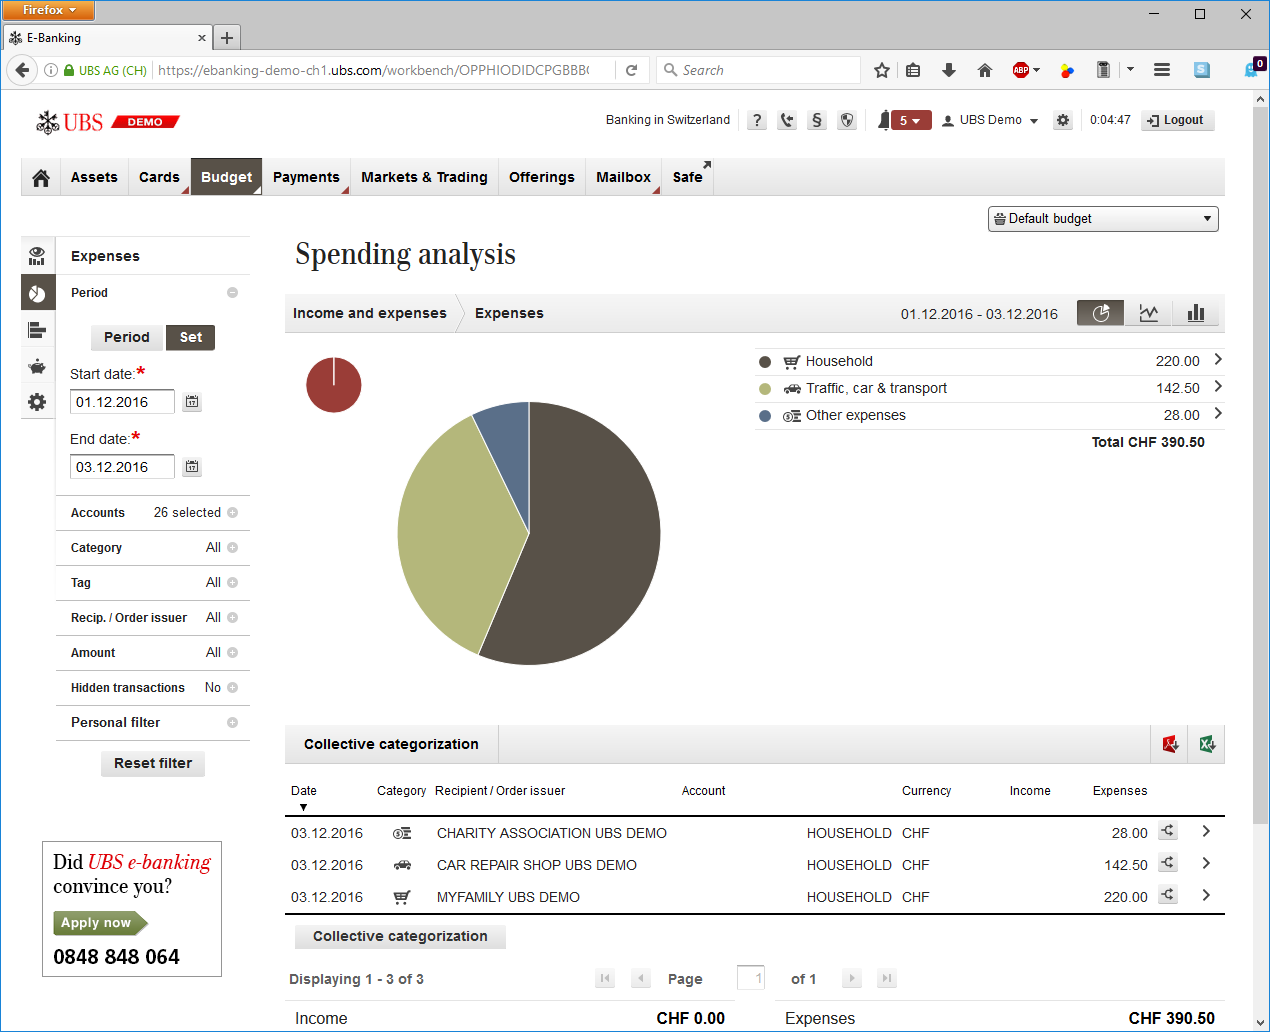
\includegraphics[width=2.8cm]{03_Figures/09_Evaluation/UBS_2_SpendingAnalysis_Filter.png}
		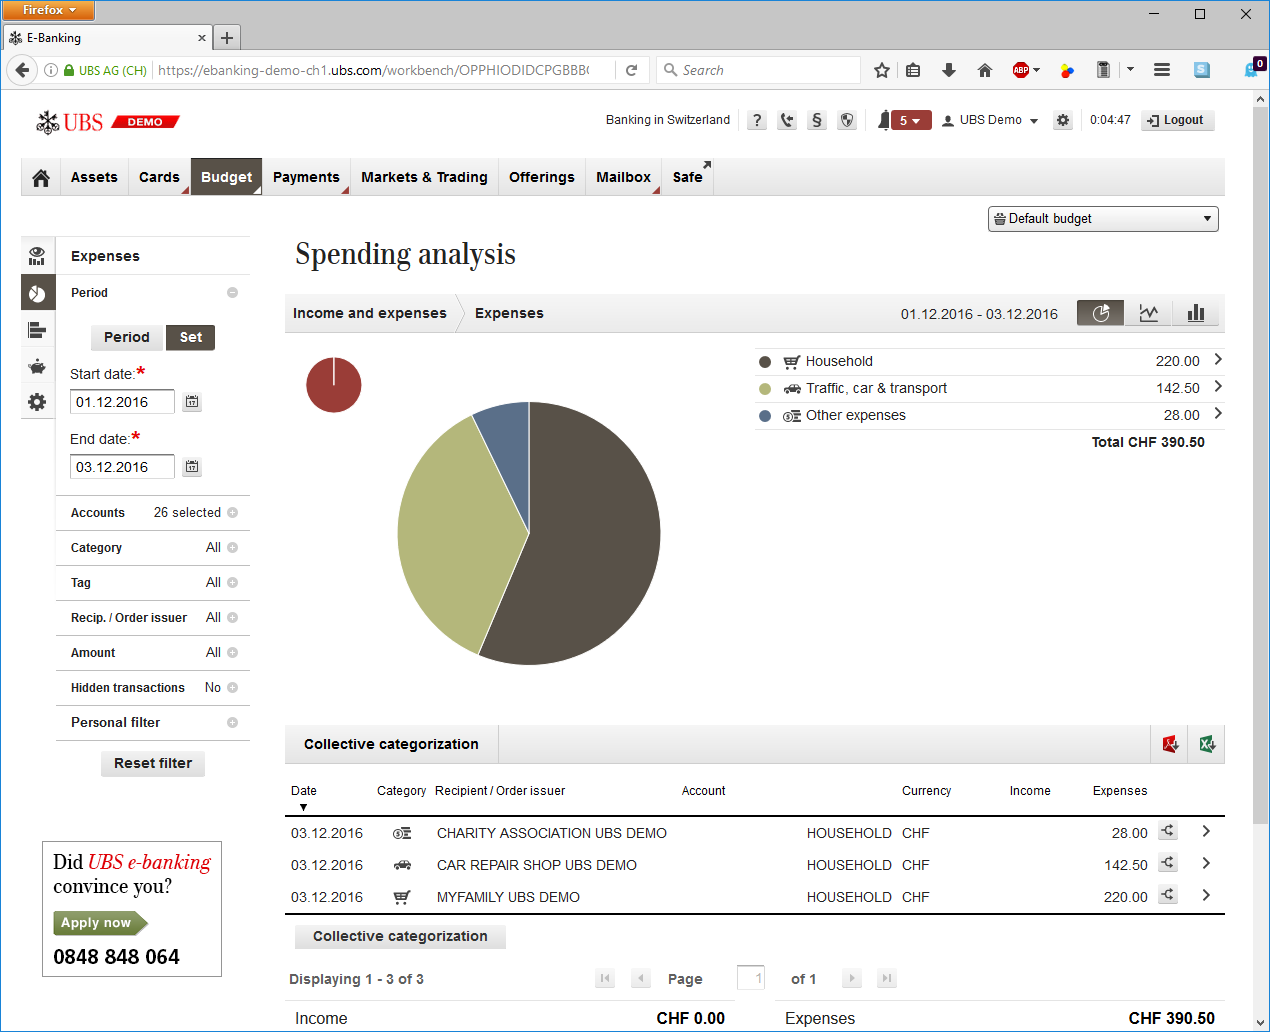
\includegraphics[width=2.8cm]{03_Figures/09_Evaluation/UBS_2_SpendingAnalysis_Filter.png}
		\caption{Visualized flow of screens in e-banking demo for Scenario 2}
		\label{fig:scenariotwoebanking}
	\end{center}
\end{figure}


\textbf{Evaluation:}  Although quite a lot of individual steps are required, the final data that is presented shows exclusively what has been searched for, and no other information. The comprehensibility however is only average as a ew additional steps are required to switch between the two years and no simultaneous view is possible. 
\begin{itemize}[noitemsep,nolistsep]
	\item Min. number of steps: \textbf{14}
	\item Exclusivity: \textbf{High}
	\item Comprehensibility: \textbf{Medium}
\end{itemize}


%-----------------------------------
%	SUBSUBSECTION 2
%-----------------------------------

\subsubsection{Prototype Application}

With the prototype application, the answer to this scenario can again be found in 3-5 interaction steps, depending on whether more detailed information from a single month is also looked at. The visualized flow for this scenario is shown in Figure \ref{fig:scenariotwoprototype}.
\begin{enumerate}[noitemsep,nolistsep]
	\item Activate "Household" category (View 4)
	\item Activate "Vacation \& travel" category (View 4)
	\item OPTIONAL: Click on a month in the Year Overview bar chart (View 1)
	\item Click on the previous year in the Year Selection (View 3)
	\item OPTIONAL: Click on a month in the Year Overview bar chart (View 1)
\end{enumerate}
\begin{figure}[h]
	\begin{center}
		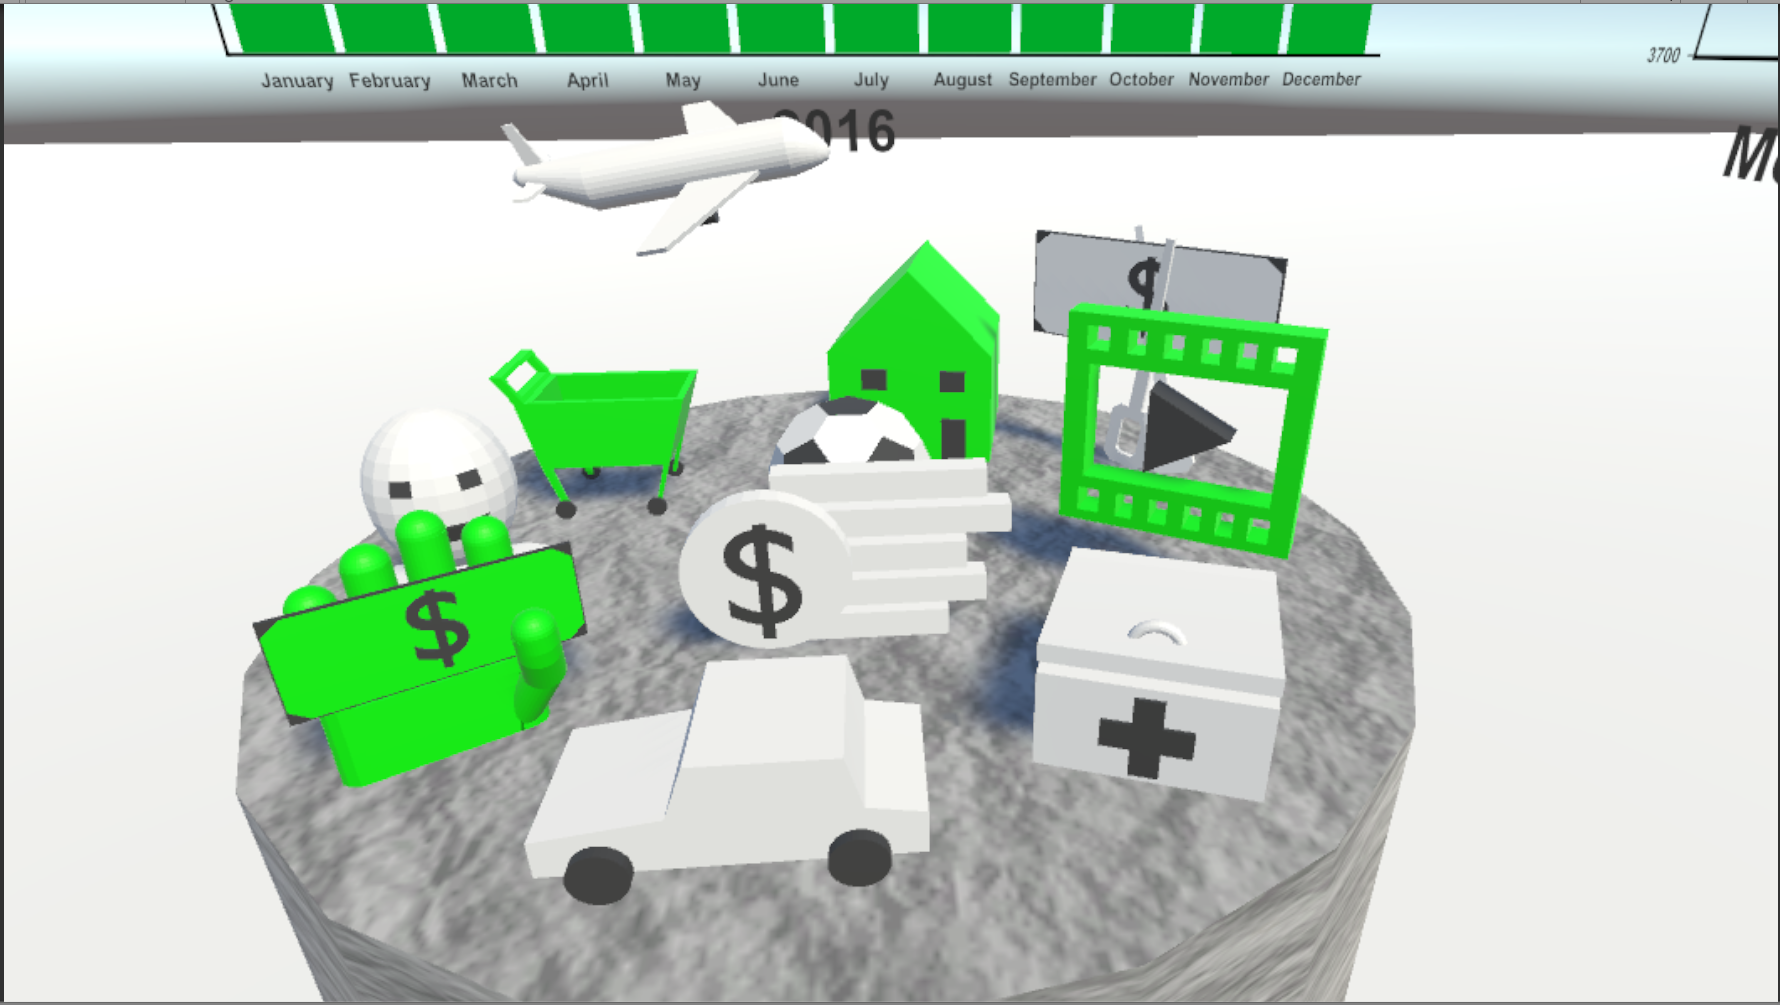
\includegraphics[width=2.8cm]{03_Figures/08_Development/View4_CategoriesFiltering.png}
		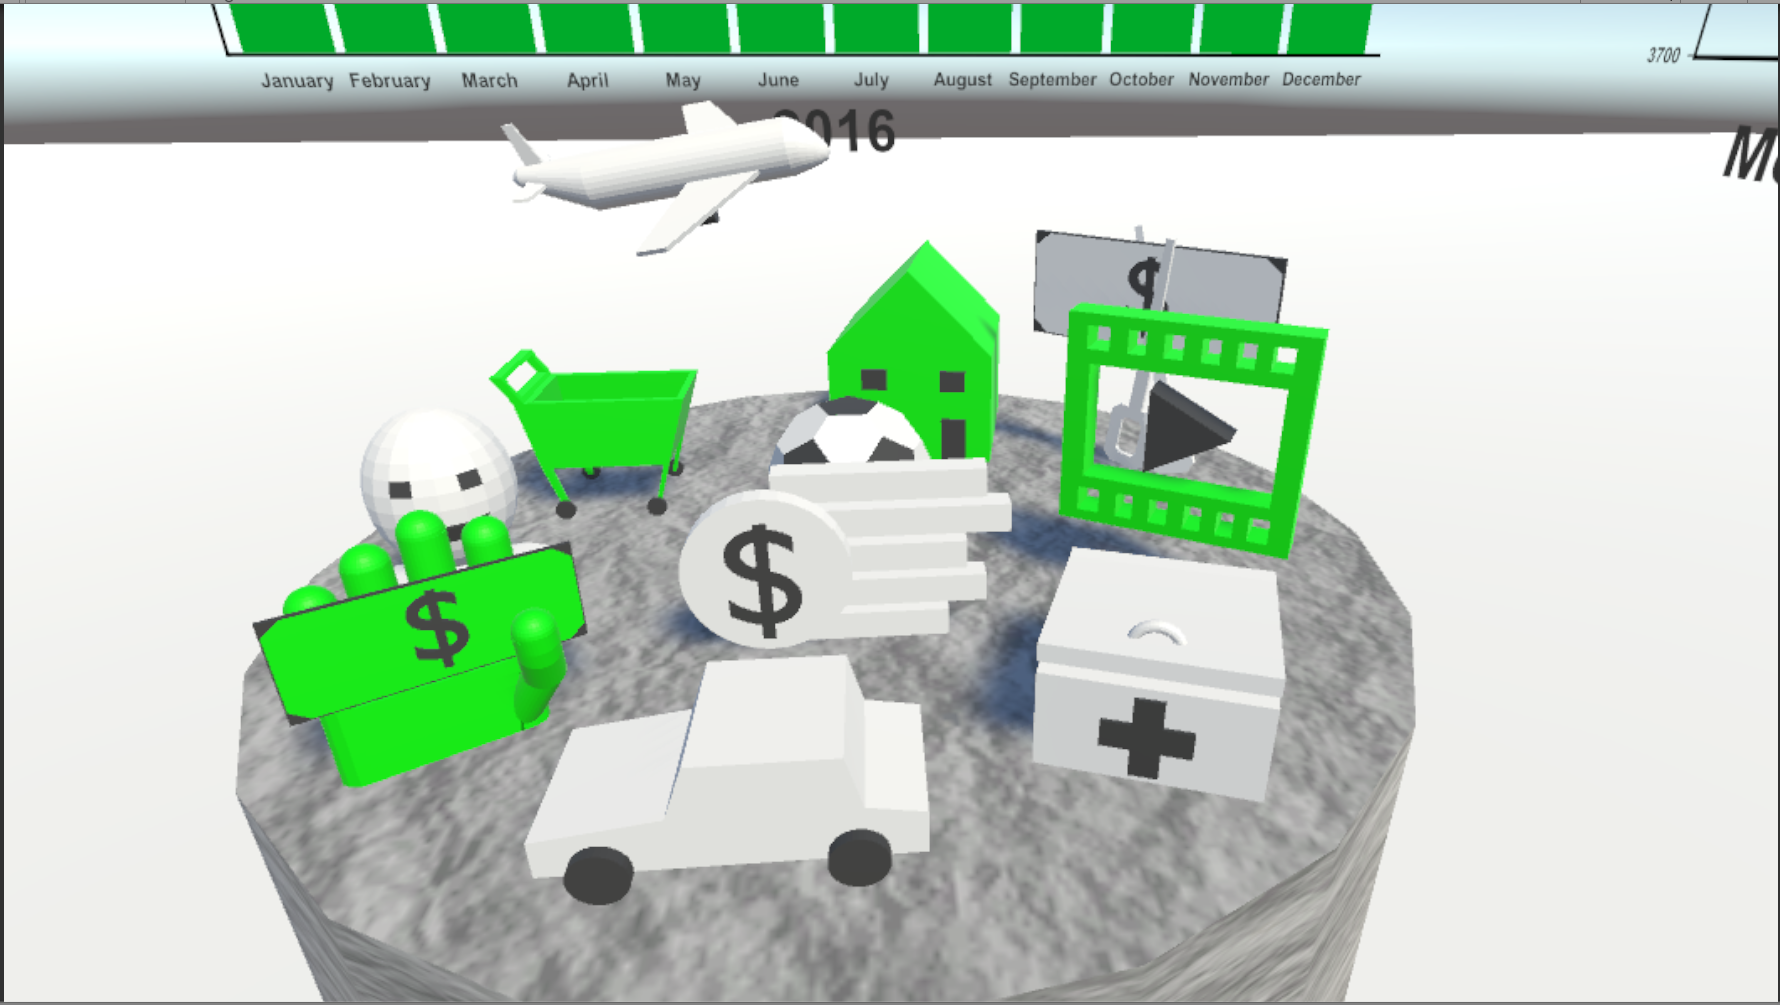
\includegraphics[width=2.8cm]{03_Figures/08_Development/View4_CategoriesFiltering.png}
		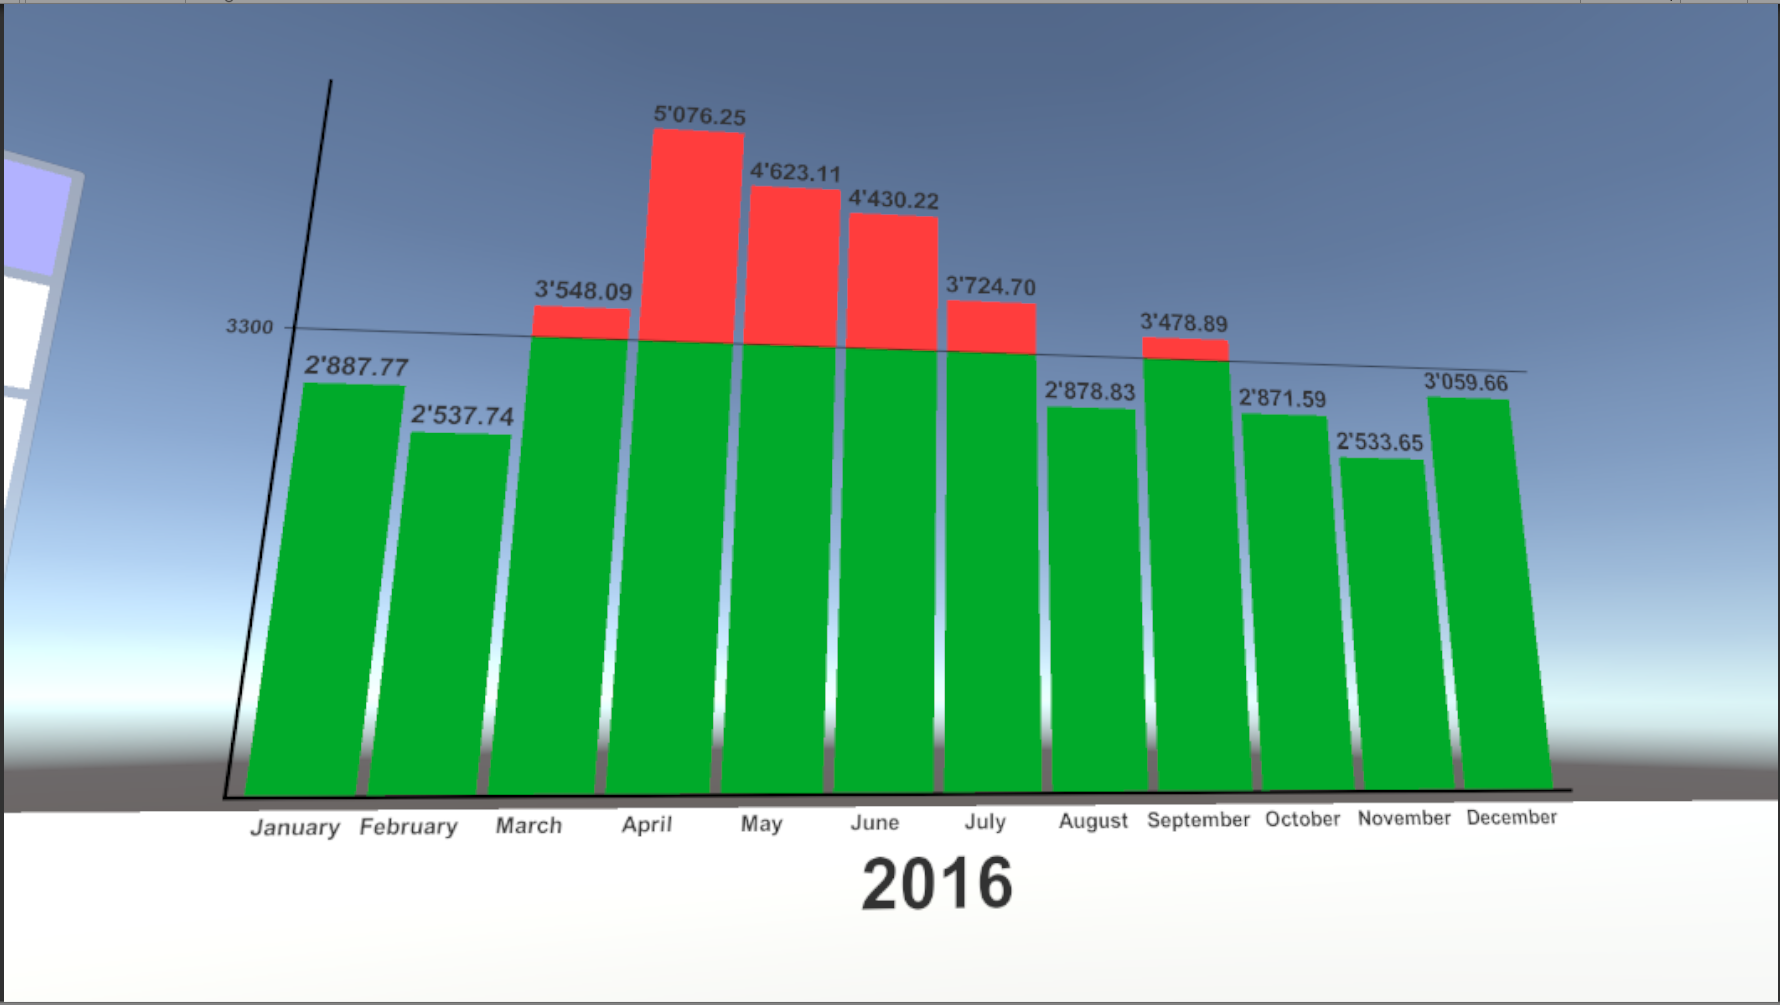
\includegraphics[width=2.8cm]{03_Figures/08_Development/View1_YearOverview.png}
		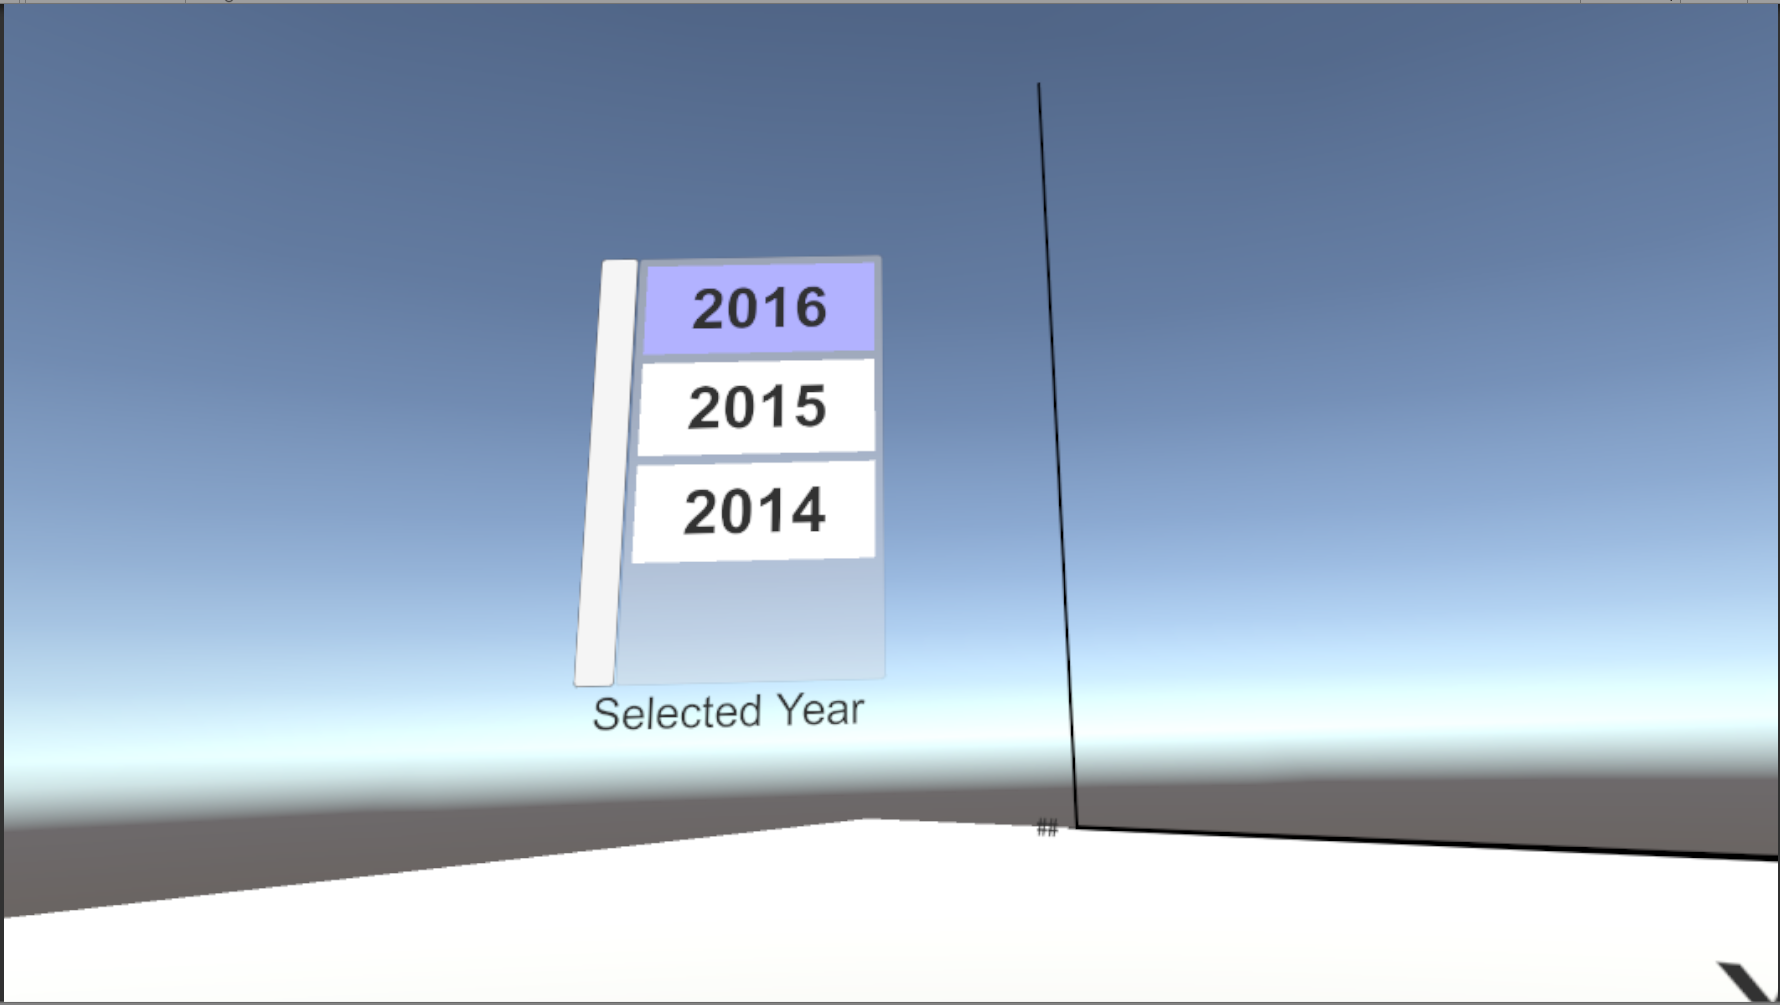
\includegraphics[width=2.8cm]{03_Figures/08_Development/View3_YearSelection.png}
		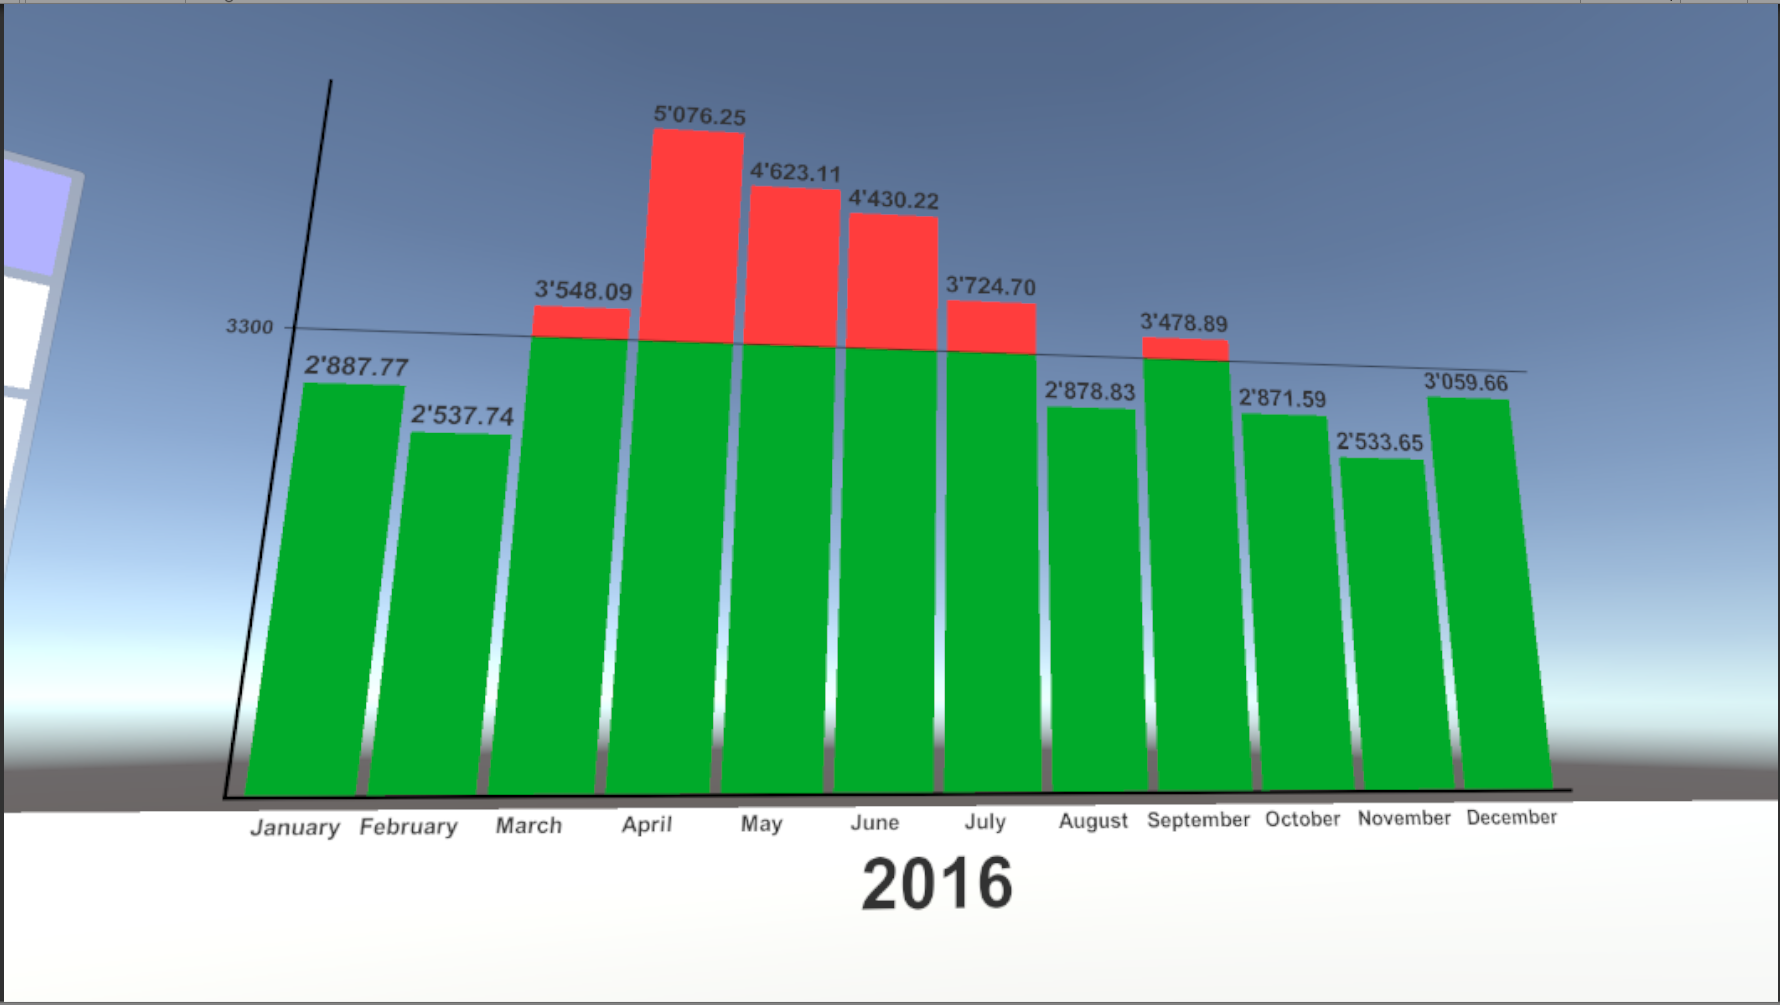
\includegraphics[width=2.8cm]{03_Figures/08_Development/View1_YearOverview.png}
		\caption{Visualized flow of views in prototype for Scenario 2}
		\label{fig:scenariotwoprototype}
	\end{center}
\end{figure}

\textbf{Evaluation:} Since the focus is on comparing the expenses for two categories over the whole course of a year, the exclusivity is high in this case with the multiple categories that can be filtered for. Also when selecting an individual month, it only shows the data of the activated categories. As for the comprehensibility, since it is not possible to have both years next to each other, switching in between them is necessary and thus requires some interpretation. Once the data has been cached, the switching between years however becomes very fast to execute.
\begin{itemize}[noitemsep,nolistsep]
	\item Min. number of steps: \textbf{3 - 5}
	\item Exclusivity: \textbf{High}
	\item Comprehensibility: \textbf{Medium}
\end{itemize}


%-----------------------------------
%	SUBSUBSECTION 1
%-----------------------------------

\subsubsection{Conclusion: Scenario 2}

In Table \ref{tbl:scenariotwocomparison} the individual evaluations of e-banking and prototype are compared with each other. The prototype application is clearly ahead of the e-banking solution in terms of the minimum amount of required steps, by almost factor three. The exclusivity and comprehensibility is similar enough to not have a clear winner between those two.
\begin{table}[h]
	\begin{center}
		\begin{tabular}{ | p{3.2cm} | p{3.8cm} | p{3.5cm} | p{2.5cm} | }
			\hline
			\textbf{Metric} & \textbf{E-Banking} & \textbf{Prototype} & \textbf{Winner} \\
			\hline
			Min. no. of steps: & 14 & 3 - 5 & Prototype \\
			\hline
			Exclusivity: & High & High & Draw \\
			\hline
			Comprehensibility: & Medium & Medium & Draw \\
			\hline
		\end{tabular}
		\caption{Scenario 2: Comparison of prototype and e-banking}
		\label{tbl:scenariotwocomparison}
	\end{center}
\end{table}


%-----------------------------------
%	SUBSECTION 3
%-----------------------------------

\subsection{Scenario 3}

\textbf{Scenario title:} \scenthree

\textbf{Exemplary situation:} Noticing that his account balance is down to zero a week before the next salary payment is expected, a user is wondering what expense(s) lead to this unexpected situation.


%-----------------------------------
%	SUBSUBSECTION 1
%-----------------------------------

\subsubsection{E-Banking}

For this scenario, the default filtering for the last 30 days helps to reduce the amount of interaction steps. Since also the current balance is always shown, in best case only 1 - 2 mouse clicks are required in order to find the data. Depending on the amount of transactions, additional filtering may be applied, or the list has to be scrolled through to find the suspicious transaction. The visualized flow for this scenario is shown in Figure \ref{fig:scenariothreeebanking}.
\begin{enumerate}[noitemsep,nolistsep]
	\item Select the desired account (1 click)
	\item OPTIONAL: Set additional filter for specific date/amount range (4 clicks)
	\item OPTIONAL: Scroll down the list of transactions if there are too many
	\item OPTIONAL: Click on the suspicious transaction in the list of Transactions (1 click)
\end{enumerate}
\begin{figure}[h]
	\begin{center}
		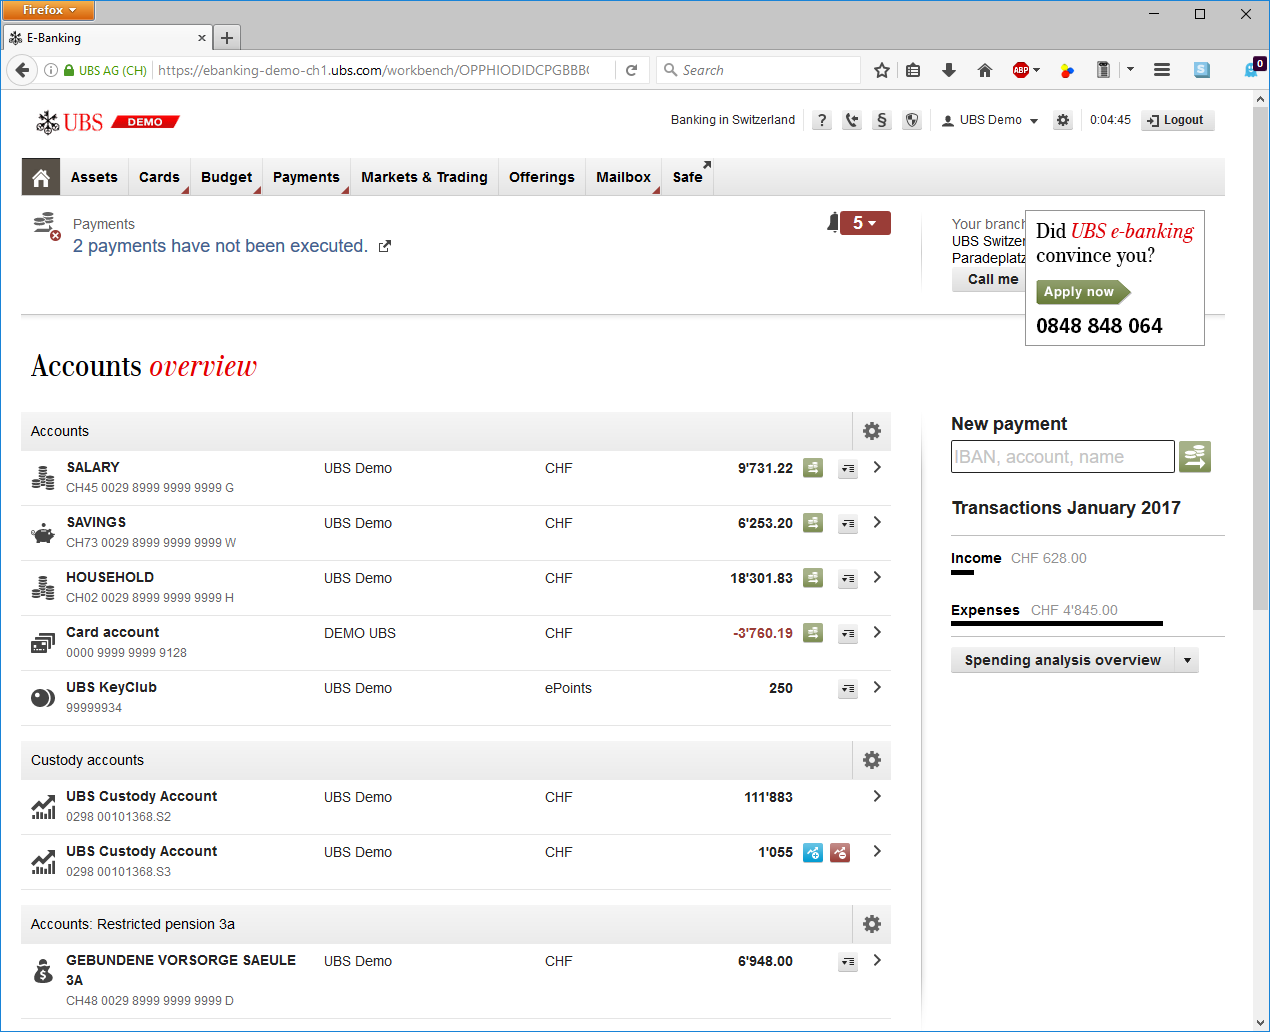
\includegraphics[width=3.5cm]{03_Figures/09_Evaluation/UBS_1_Overview.png}
		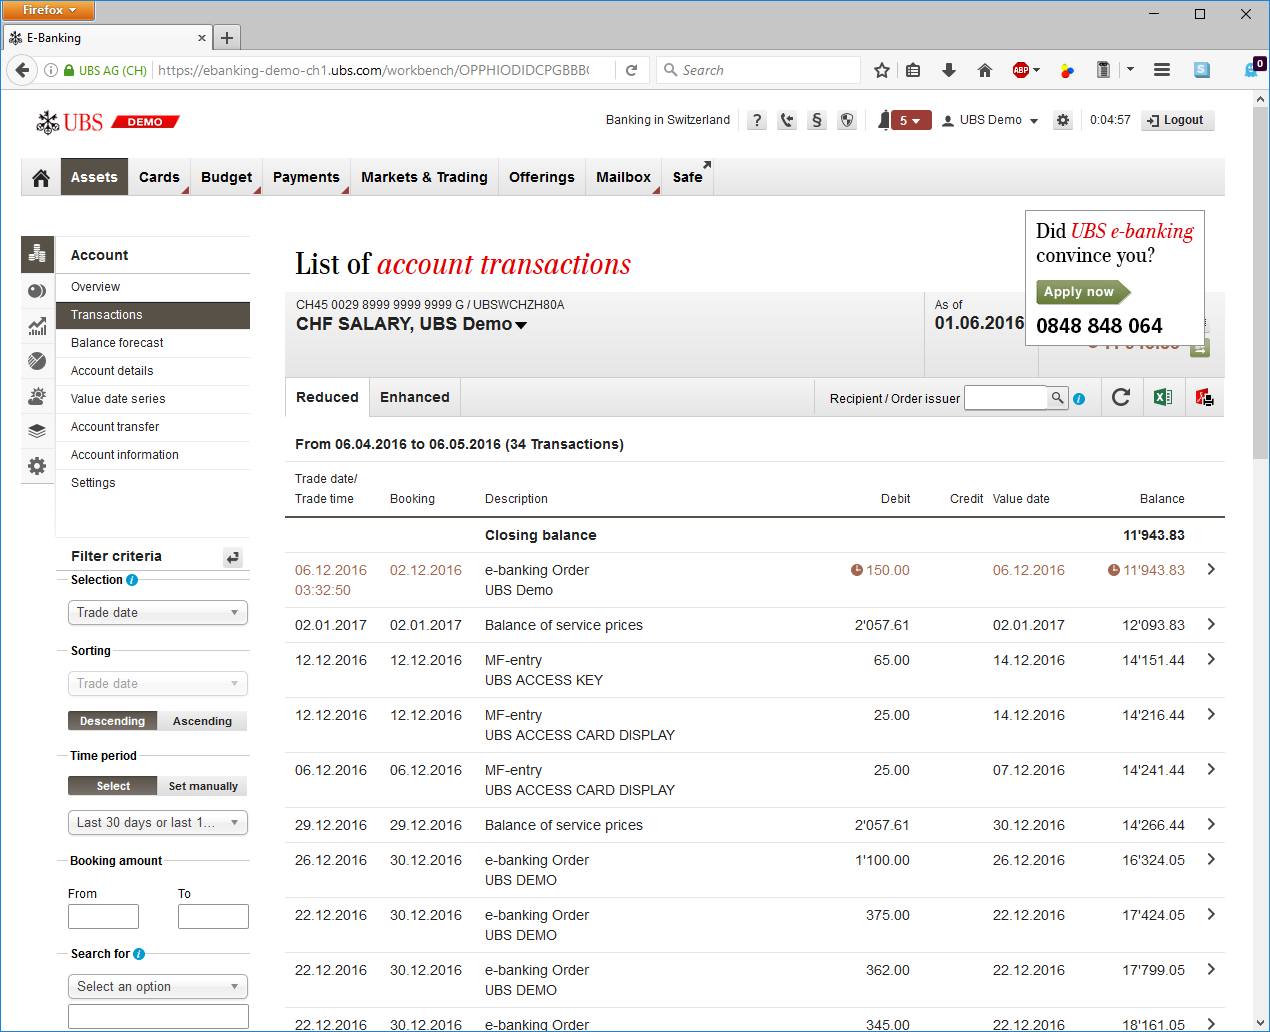
\includegraphics[width=3.5cm]{03_Figures/09_Evaluation/UBS_3_AccountTransactions.png}
		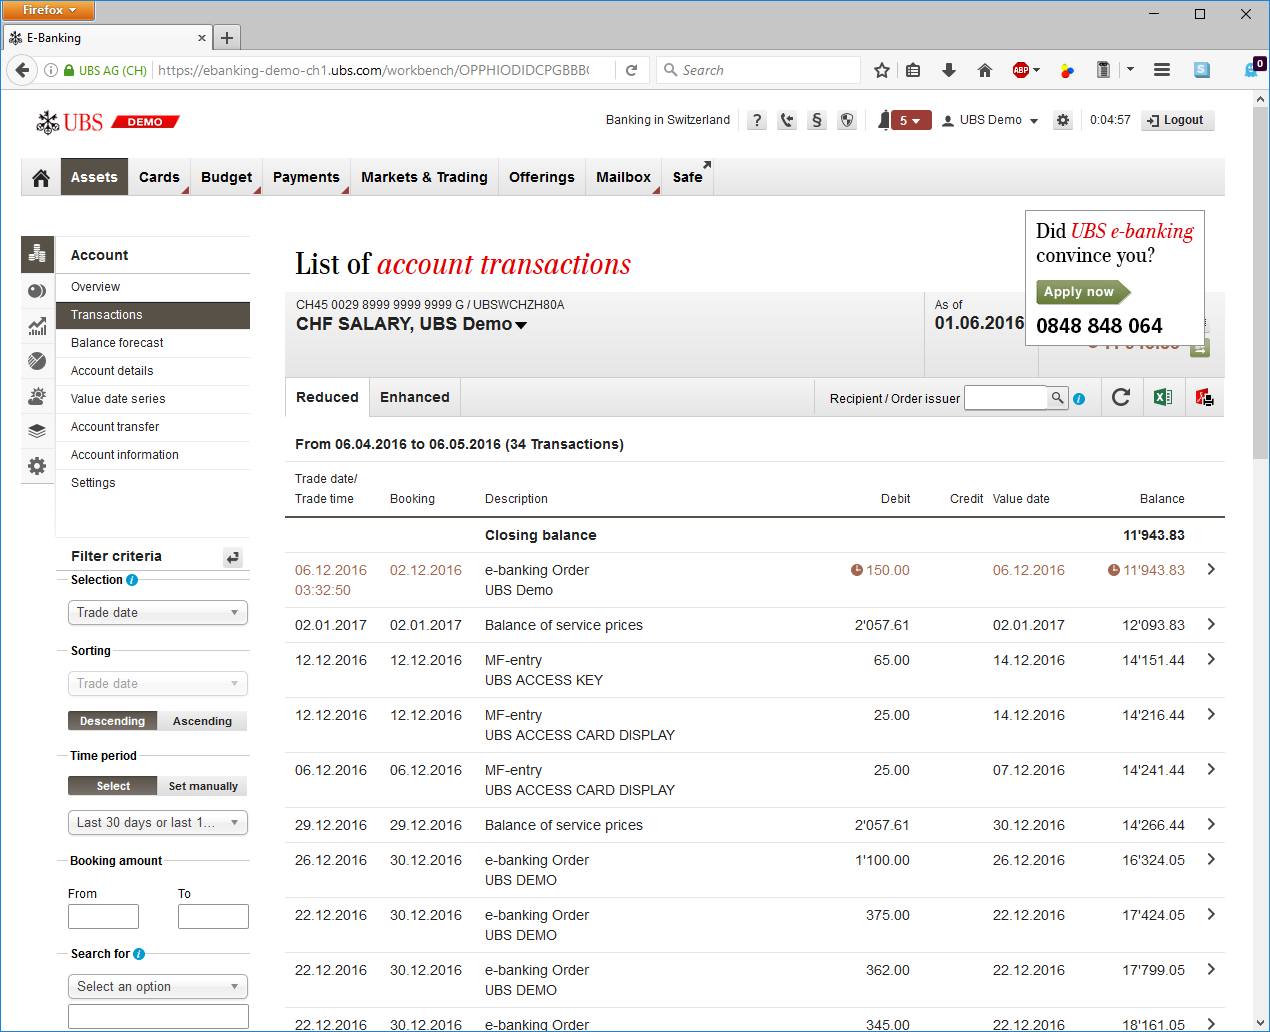
\includegraphics[width=3.5cm]{03_Figures/09_Evaluation/UBS_3_AccountTransactions.png}
		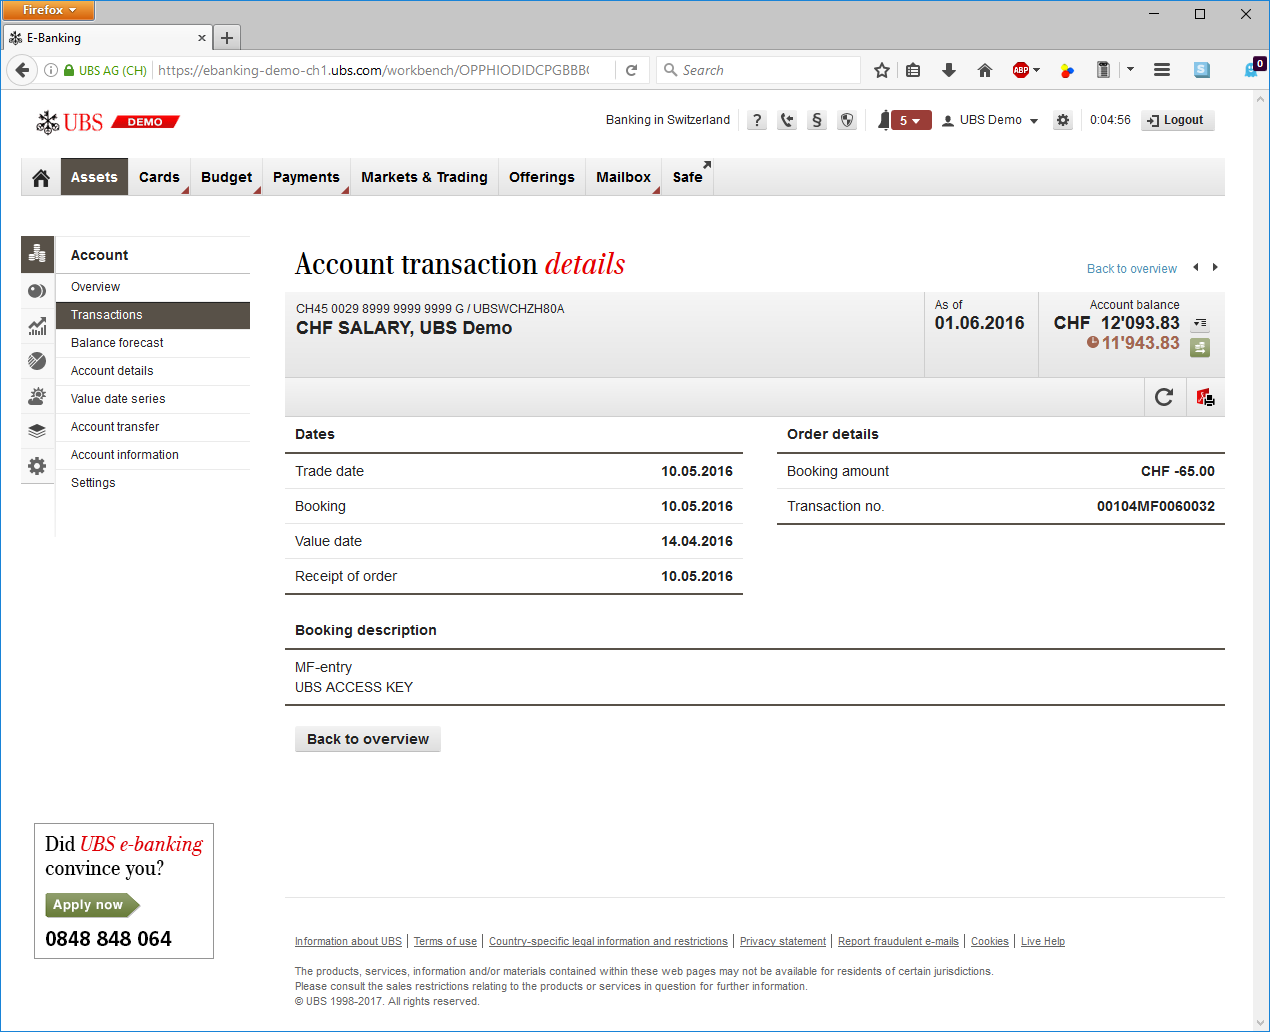
\includegraphics[width=3.5cm]{03_Figures/09_Evaluation/UBS_4_AccountTransactionDetails.png}
		\caption{Visualized flow of screens in e-banking demo for Scenario 3}
		\label{fig:scenariothreeebanking}
	\end{center}
\end{figure}

\textbf{Evaluation:} The default filtering helps to directly achieve an average exclusivity of the presented data, whereas with an additional filter it can be narrowed to almost exclusively to the root cause of the unexpected high expenses. The comprehensibility also is very high since the current account balance is shown together with the transaction amount, which makes the understanding of the data much simpler.
\begin{itemize}[noitemsep,nolistsep]
	\item Min. number of steps: \textbf{1 - 6}
	\item Exclusivity: \textbf{High} (with filtered day), \textbf{Medium} (without)
	\item Comprehensibility: \textbf{High}
\end{itemize}


%-----------------------------------
%	SUBSUBSECTION 2
%-----------------------------------

\subsubsection{Prototype Application}

The answer to this scenario can be found with only 2-5 interaction steps in the prototype application, depending how spread out the suspicious payments were over the selected month. The visualized flow for this scenario is shown in Figure \ref{fig:scenariothreeprototype}.
\begin{enumerate}[noitemsep,nolistsep]
	\item Toggle-activate all categories (View 4)
	\item Click on the current month in the Year Overview bar chart (View 1)
	\item OPTIONAL: Click on a day with a big jump in expenses in the Month Overview bar chart (View 2)
	\item OPTIONAL: Scroll down the list of transactions if there are too many (View 5)
	\item OPTIONAL: Click on the suspicious transaction in the List of Transactions (View 5)
\end{enumerate}
\begin{figure}[h]
	\begin{center}
		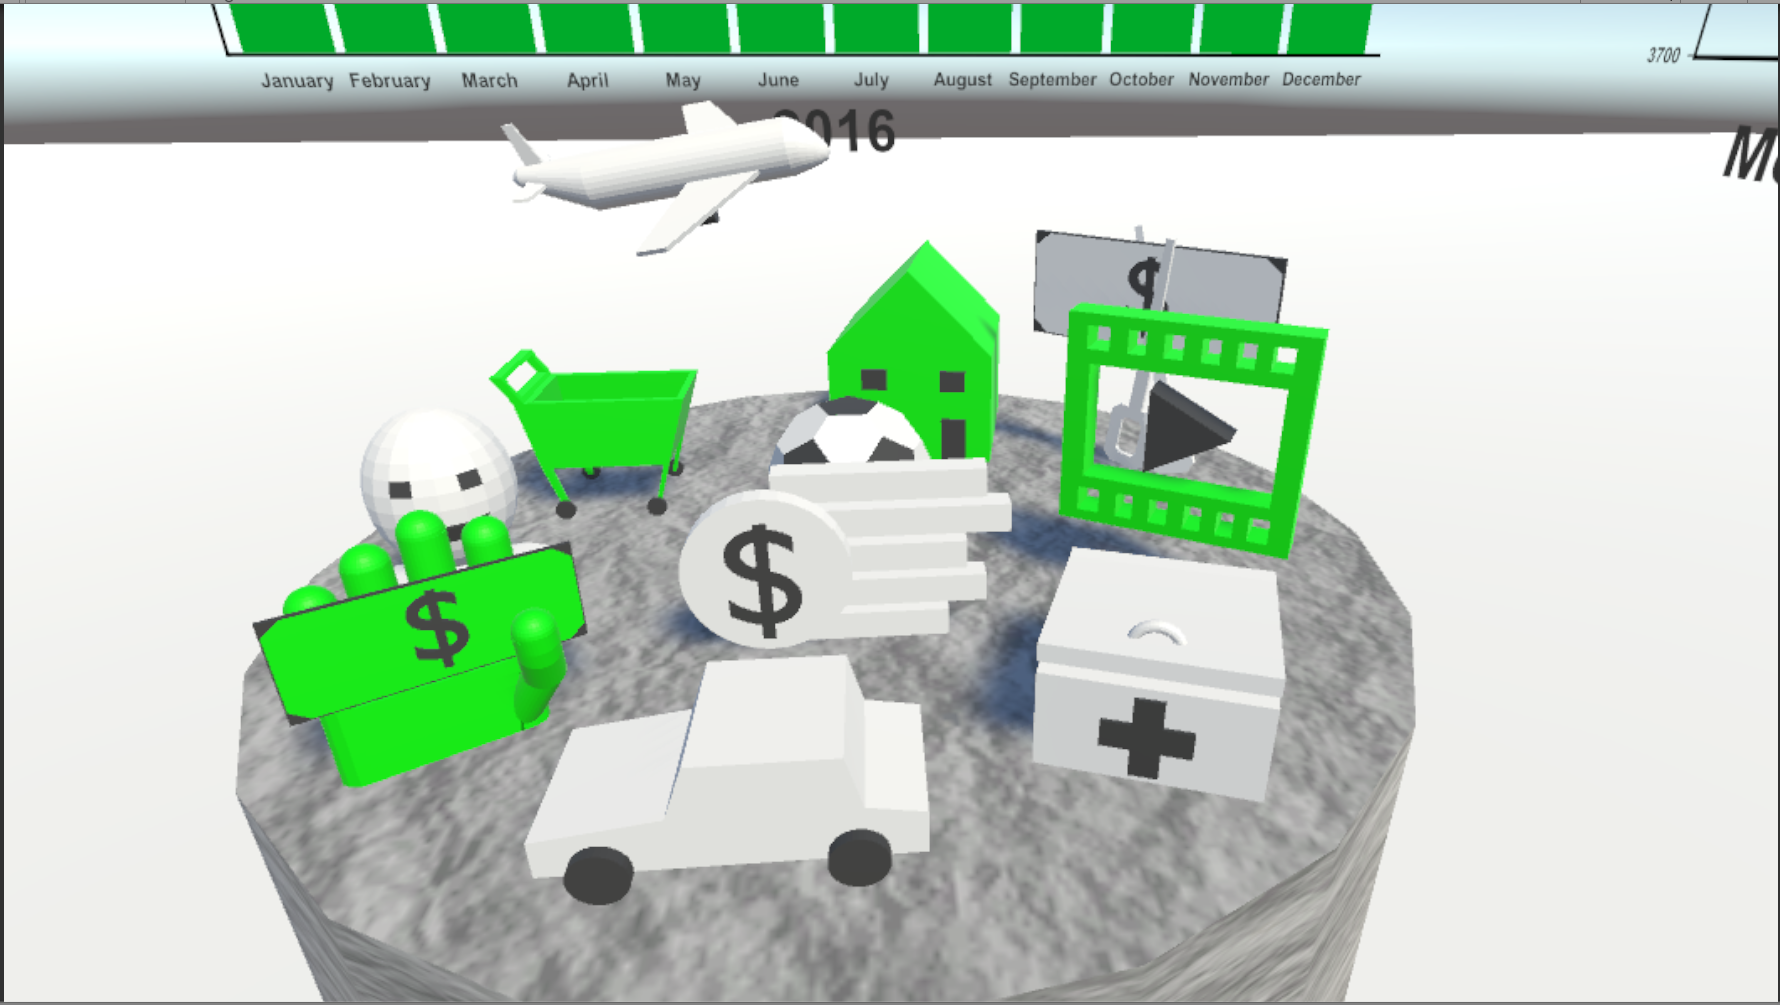
\includegraphics[width=2.8cm]{03_Figures/08_Development/View4_CategoriesFiltering.png}
		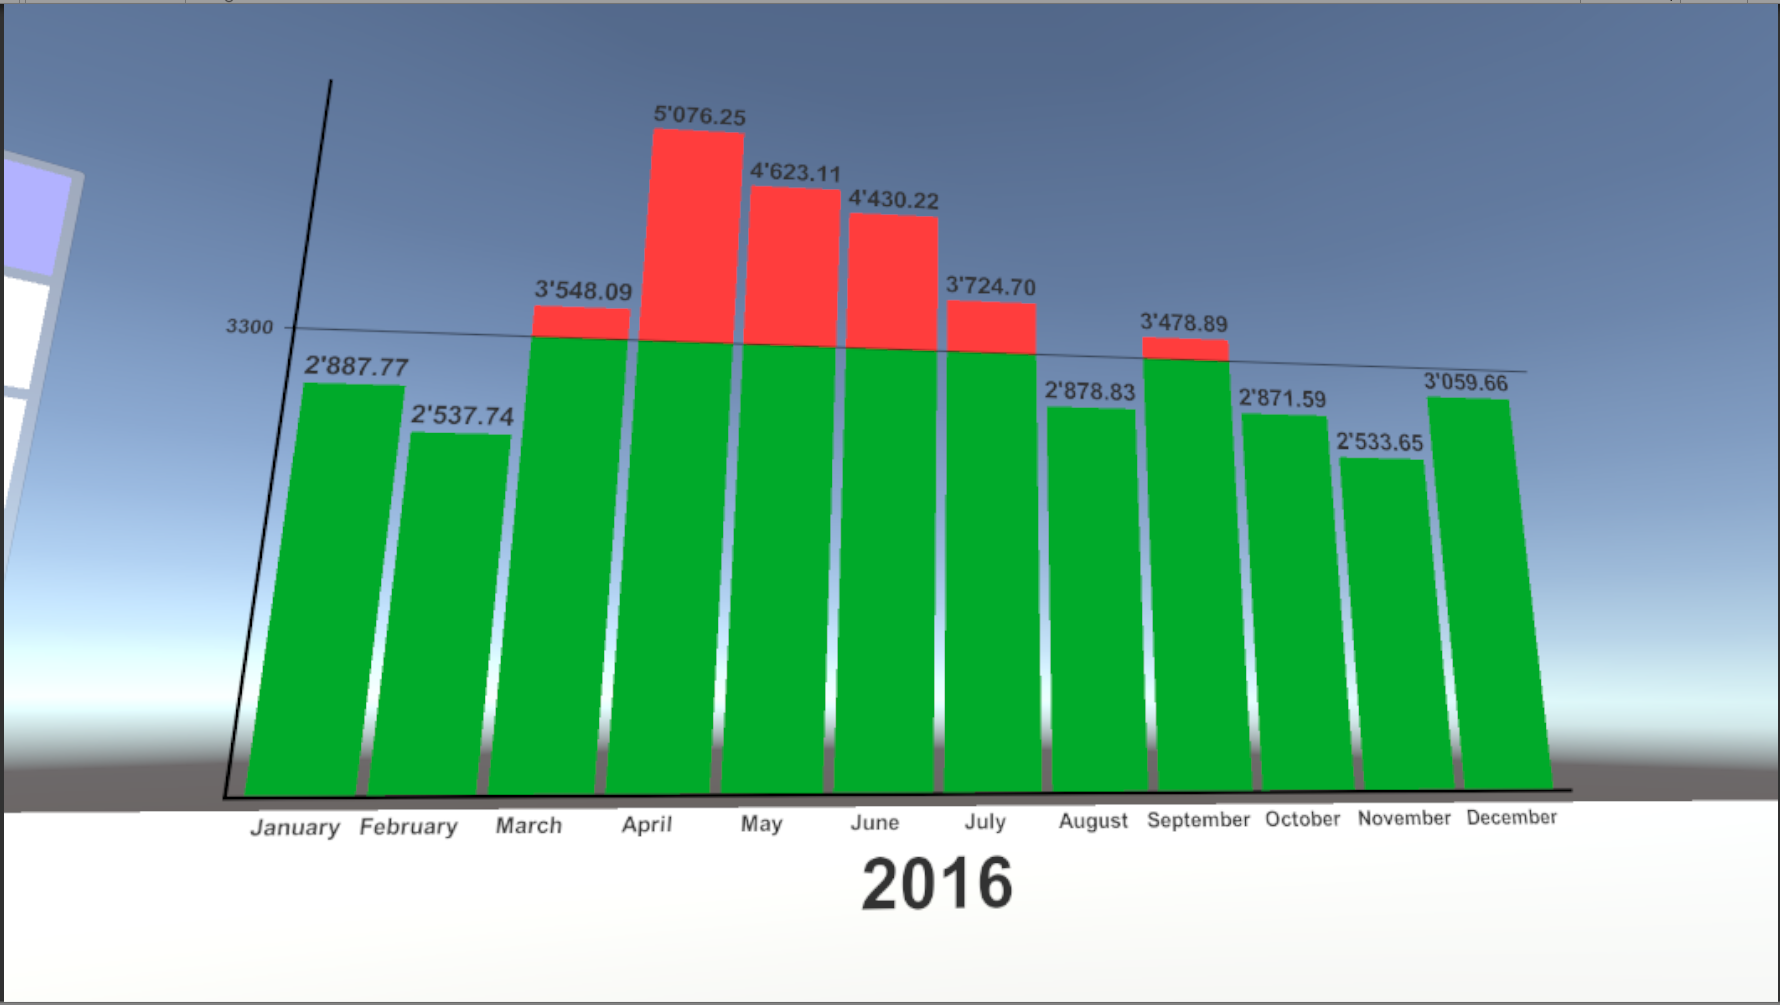
\includegraphics[width=2.8cm]{03_Figures/08_Development/View1_YearOverview.png}
		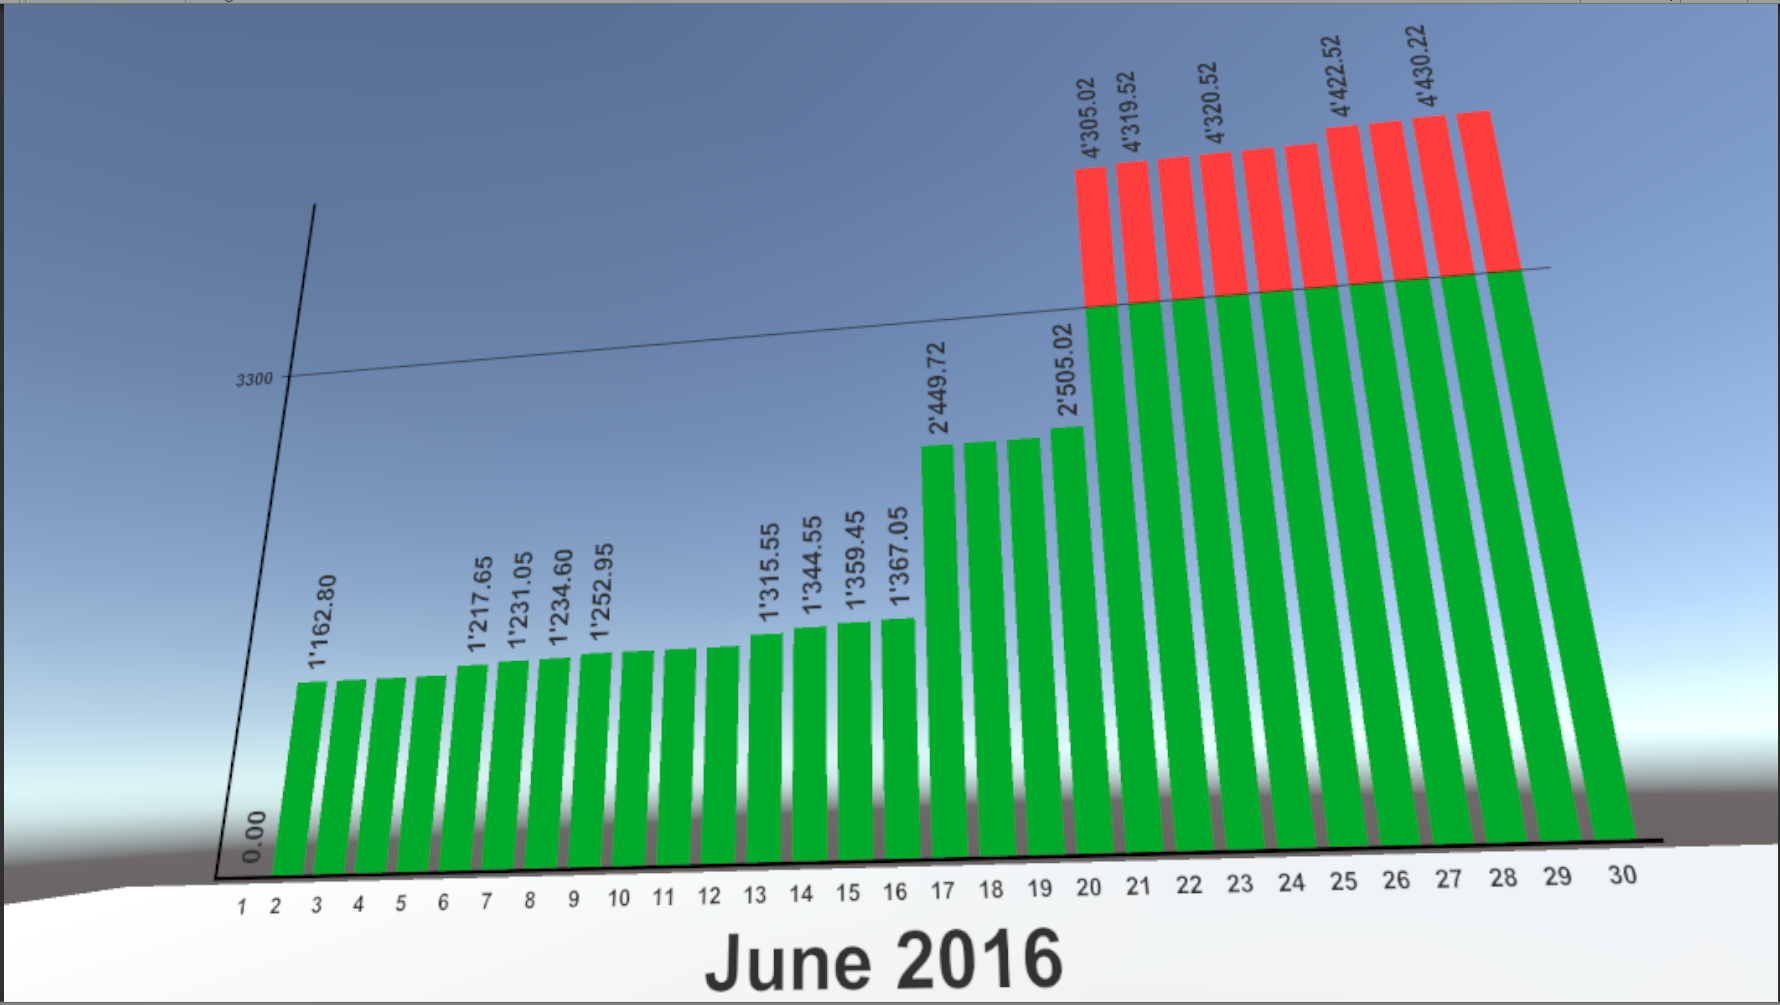
\includegraphics[width=2.8cm]{03_Figures/08_Development/View2_MonthOverview.png}
		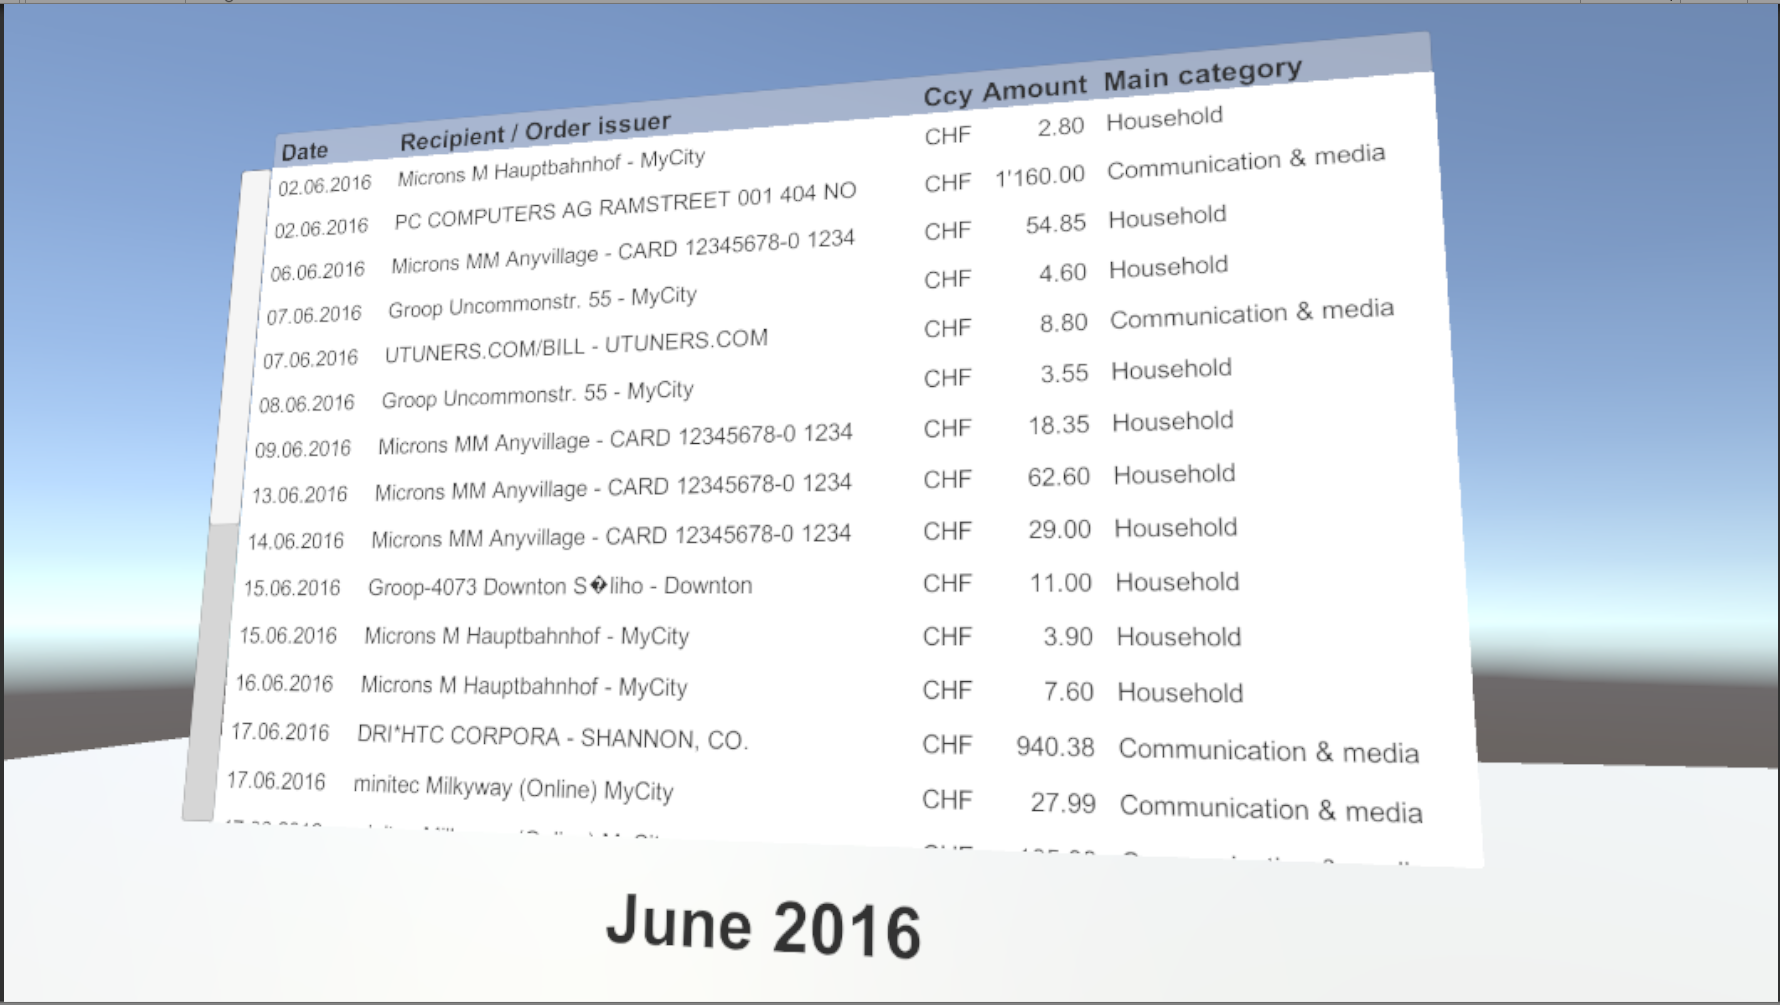
\includegraphics[width=2.8cm]{03_Figures/08_Development/View5_FinTransactionsOverview.png}
		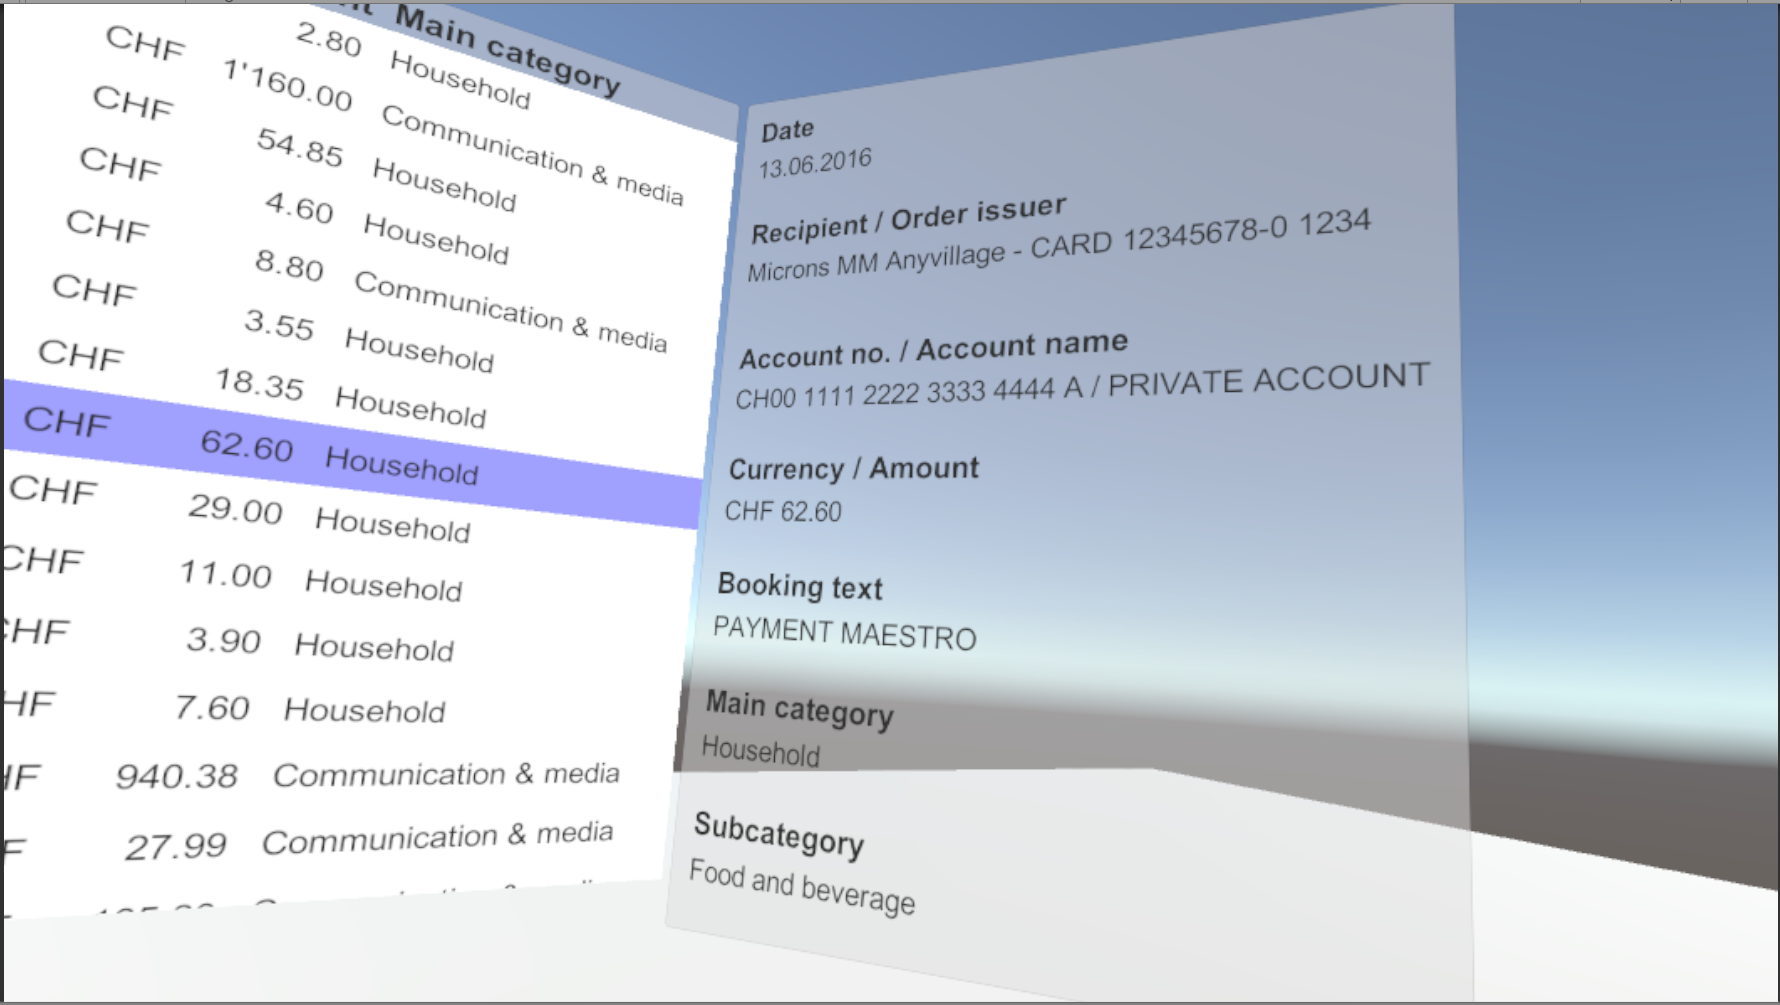
\includegraphics[width=2.8cm]{03_Figures/08_Development/View6_FinTransactionDetails.png}
		\caption{Visualized flow of views in prototype for Scenario 3}
		\label{fig:scenariothreeprototype}
	\end{center}
\end{figure}

\textbf{Evaluation:} When all categories are activated, the Month Overview should give a clear indication on which day(s) unexpected high transactions were executed. If it focuses on a single day, it can be selected and then the table shows only this very specific transactions, leading to a medium exclusivity. If it is however more spread out over the whole month, the exclusivity is rather low. From a comprehensibility aspect, the user is still required to go through the list and and find the suspicious transactions by himself.
\begin{itemize}[noitemsep,nolistsep]
	\item Min. number of steps: \textbf{2 - 5}
	\item Exclusivity: \textbf{Medium} (with filtered day), \textbf{Low} (without)
	\item Comprehensibility: \textbf{Medium}
\end{itemize}


%-----------------------------------
%	SUBSUBSECTION 1
%-----------------------------------

\subsubsection{Conclusion: Scenario 3}

A comparison of e-banking and the prototype for the third scenario is shown in Table \ref{tbl:scenariothreecomparison}. In terms of minimum required amount of steps, both applications are very close to each other and none of them is clearly better than the other one. For the other two metrics, the e-banking is the clear winner due to its much more detailed filtering option that is available and the more dynamic presentation of the data via the account specific view that does not exist in the prototype.
\begin{table}[h]
	\begin{center}
		\begin{tabular}{ | p{3.2cm} | p{3.8cm} | p{3.5cm} | p{2.5cm} | }
			\hline
			\textbf{Metric} & \textbf{E-Banking} & \textbf{Prototype} & \textbf{Winner} \\
			\hline
			Min. no. of steps: & 1 - 6 & 2 - 5 & Draw \\
			\hline
			Exclusivity: & High & Medium / Low & E-Banking \\
			\hline
			Comprehensibility: & High & Medium & E-Banking \\
			\hline
		\end{tabular}
		\caption{Scenario 3: Comparison of prototype and e-banking}
		\label{tbl:scenariothreecomparison}
	\end{center}
\end{table}


%-----------------------------------
%	SUBSECTION 4
%-----------------------------------

\subsection{Scenario 4}

\textbf{Scenario title:} \scenfour

\textbf{Exemplary situation:} Since only working part-time now, a user has to pay more close attention to not exceed his smaller monthly budget for household, personal expenses, entertainment, and his hobbies. He wants to see in advance where he currently is at and whether there is some budget left at the end of the month.


%-----------------------------------
%	SUBSUBSECTION 1
%-----------------------------------

\subsubsection{E-Banking}

Enabling the filter for the four categories requires some additional steps, as well as the filter for the date range which is required in this situation. The default filter of the last 30 days will provide wrong information about the monthly expenses and thus first has to be adjusted manually. Afterwards, a summary of the expenses for the date range and category selection is presented alongside a list of all transactions within this filter set. The visualized flow for this scenario is shown in Figure \ref{fig:scenariofourebanking}.
\begin{enumerate}[noitemsep,nolistsep]
	\item Go via "Budget" to "Expenses" (2 clicks)
	\item Set filter for the four categories (6 clicks)
	\item Set filter for specific date range in current year (4 clicks)
	\item OPTIONAL: Scroll down the list of transactions if there are too many
\end{enumerate}
\begin{figure}[h]
	\begin{center}
		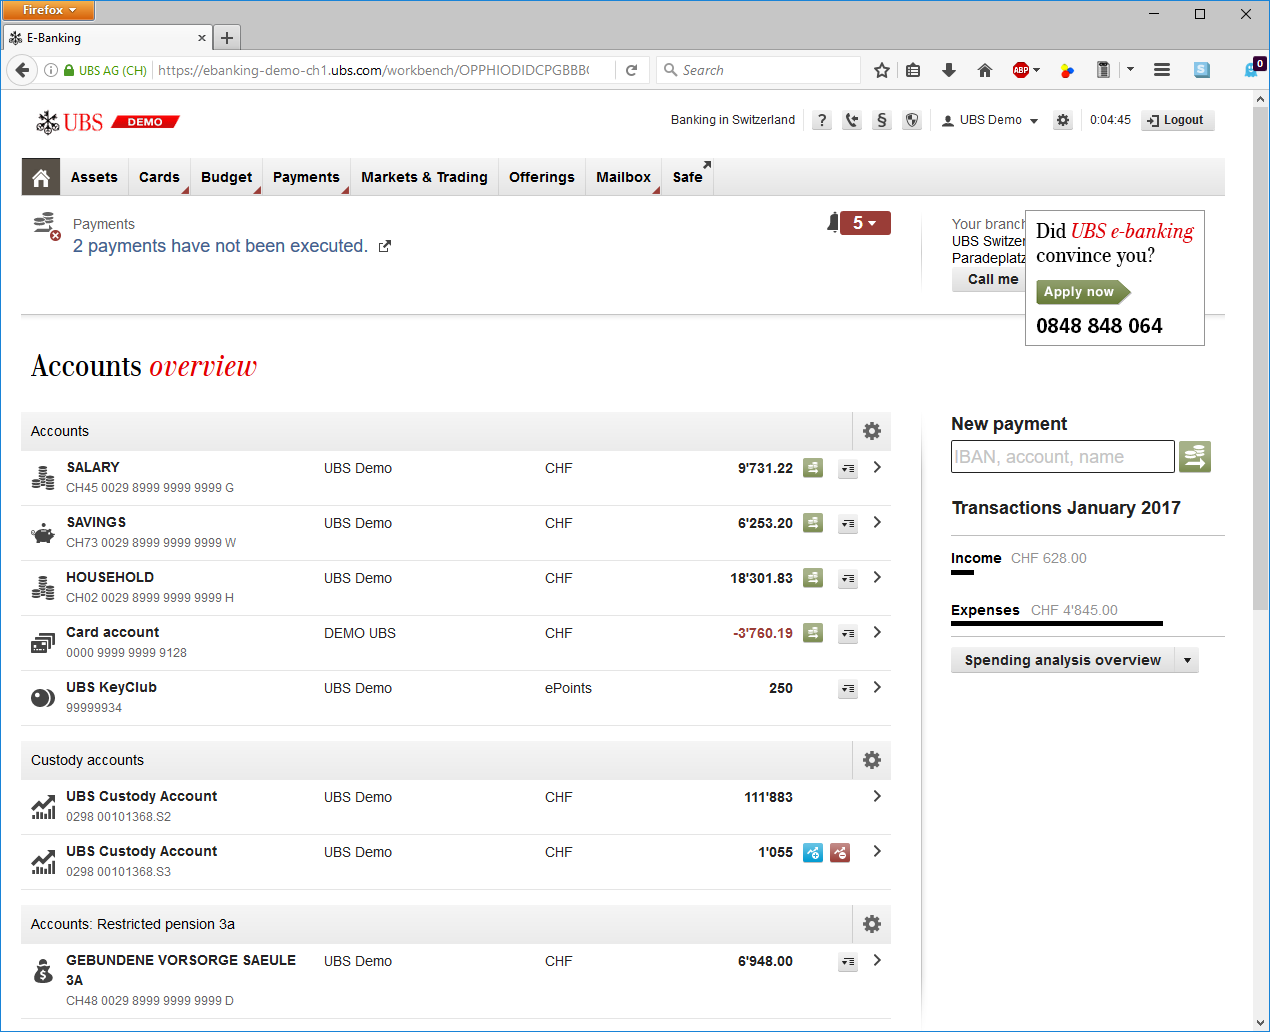
\includegraphics[width=3.5cm]{03_Figures/09_Evaluation/UBS_1_Overview.png}
		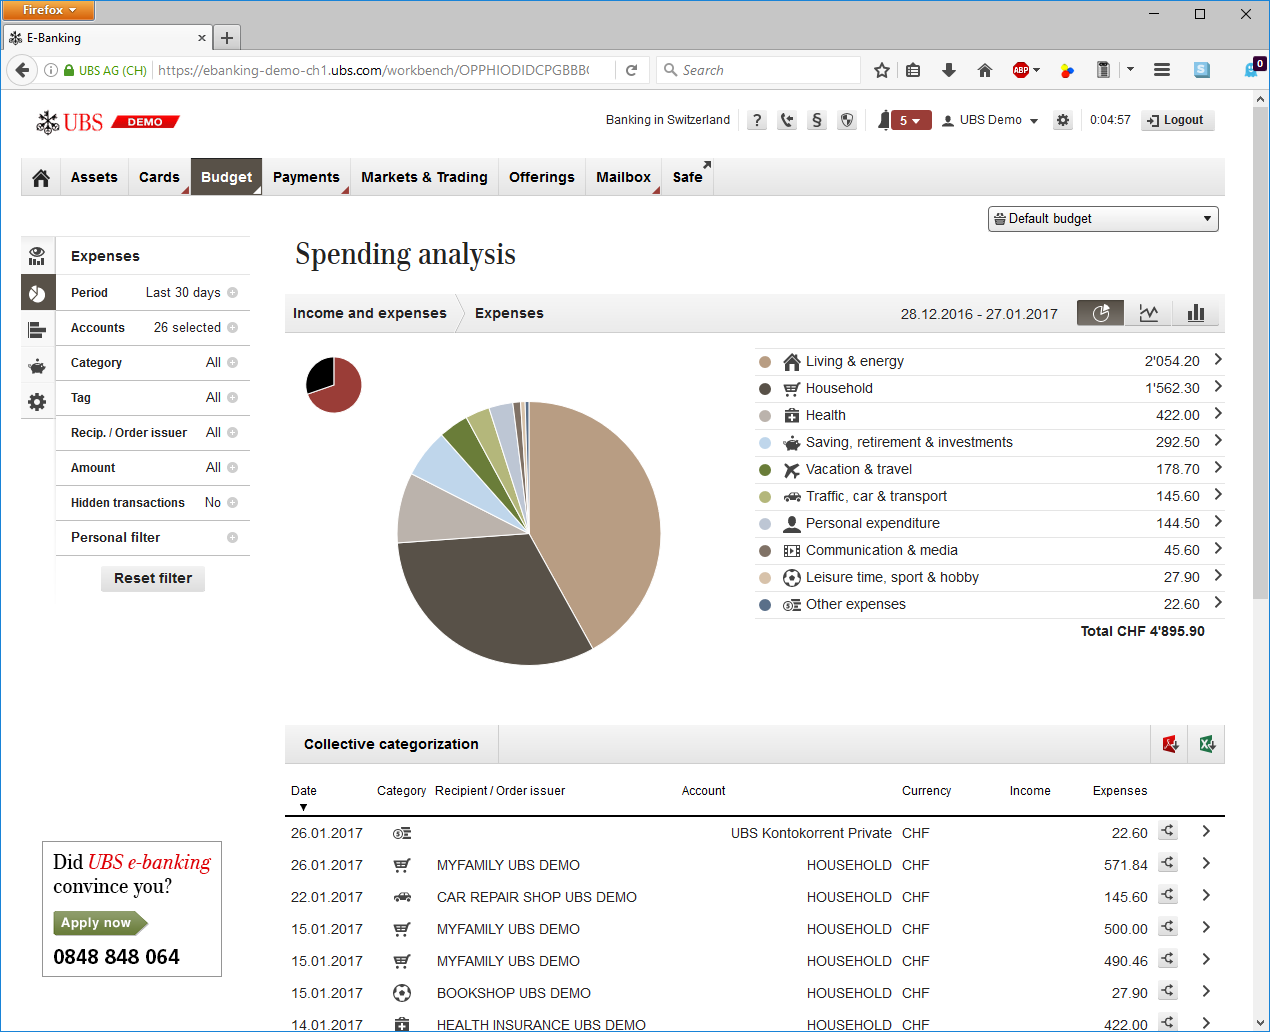
\includegraphics[width=3.5cm]{03_Figures/09_Evaluation/UBS_2_SpendingAnalysis.png}
		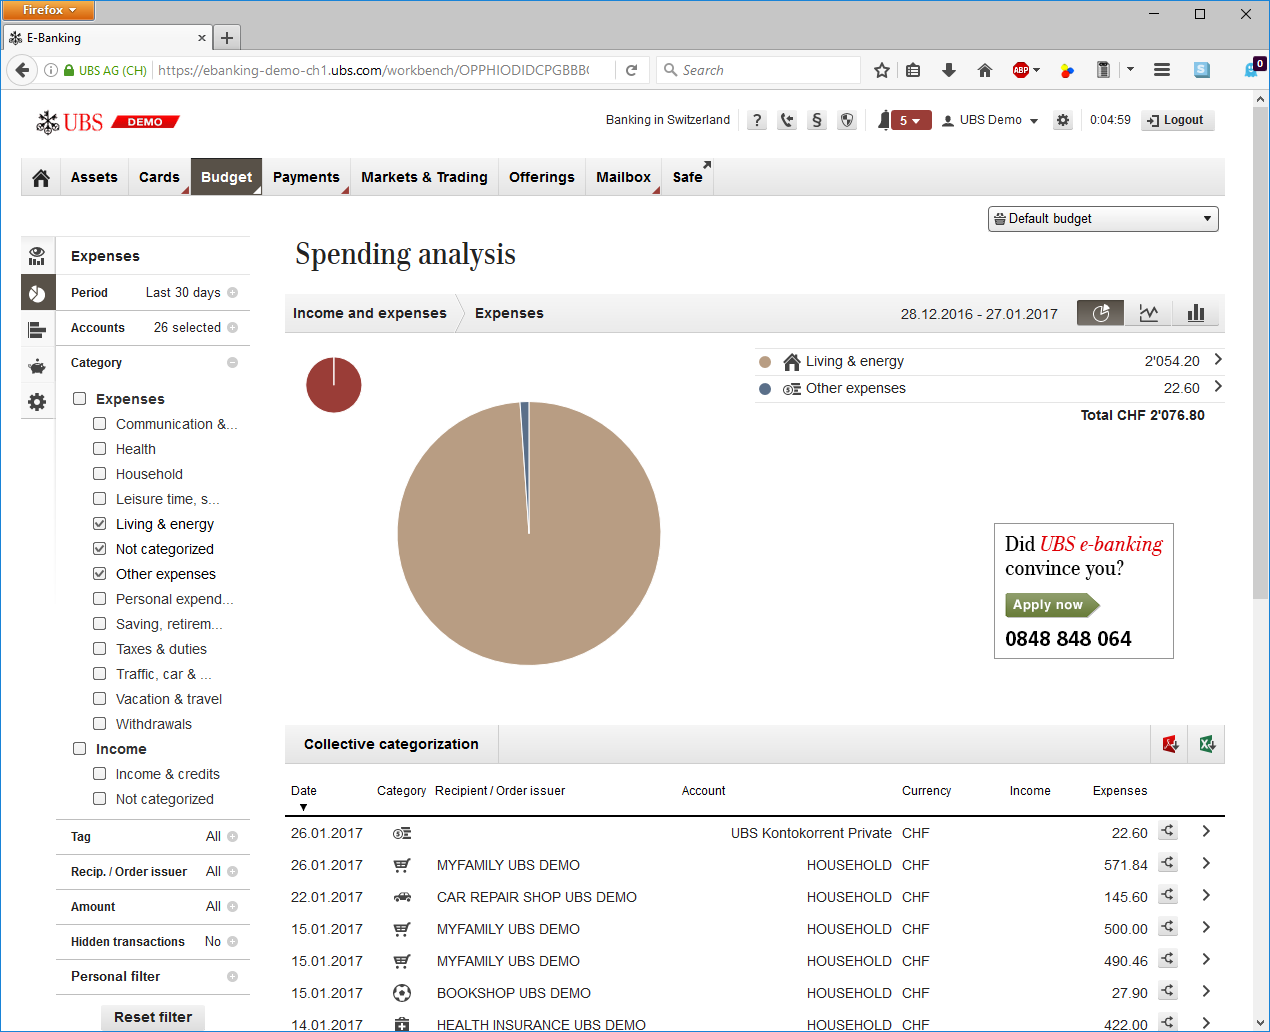
\includegraphics[width=3.5cm]{03_Figures/09_Evaluation/UBS_2_SpendingAnalysis_FilterCat.png}
		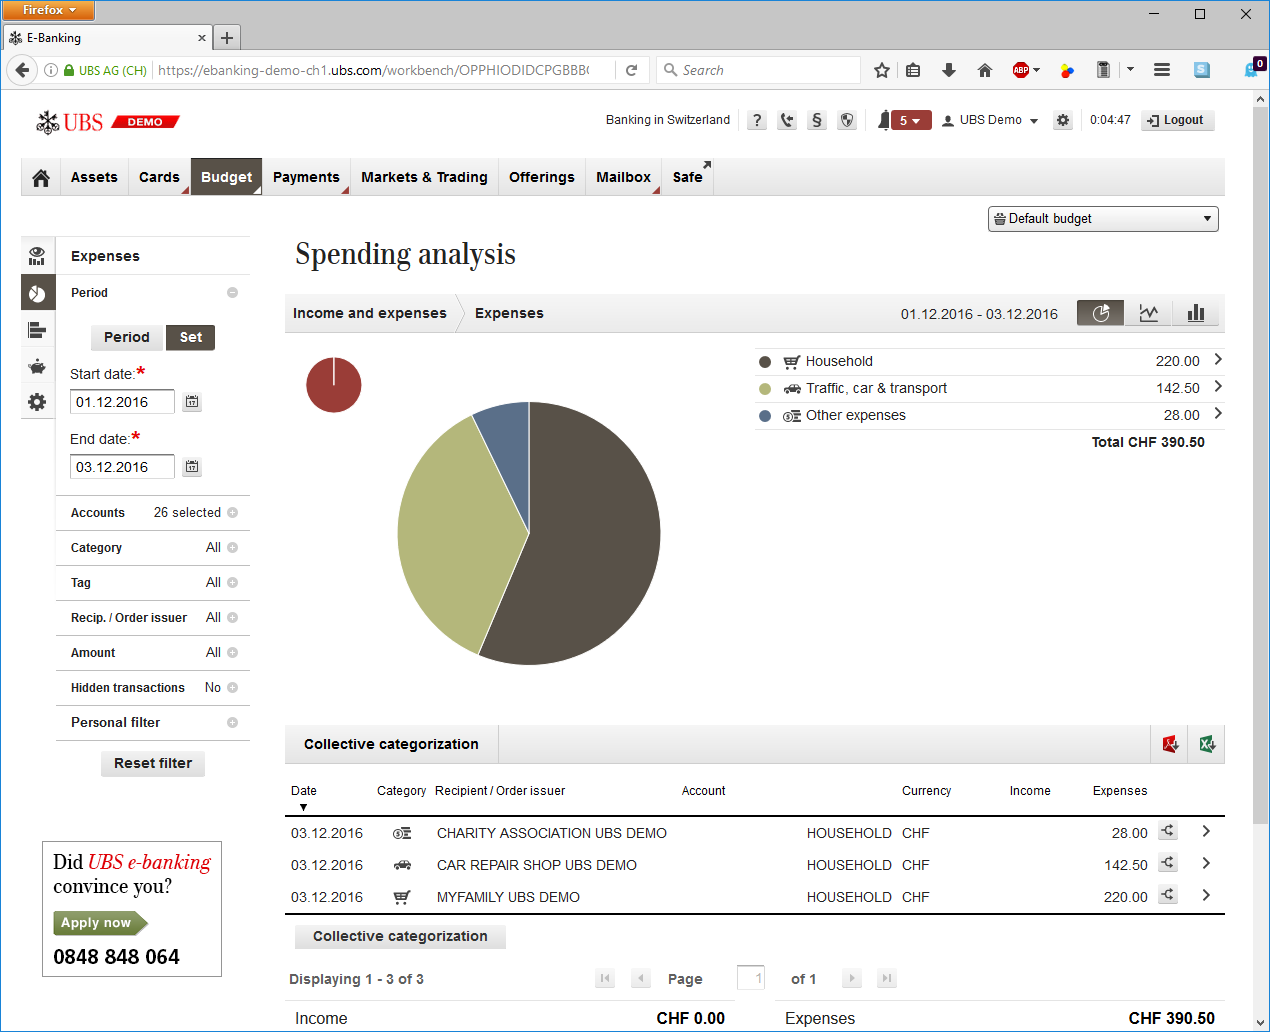
\includegraphics[width=3.5cm]{03_Figures/09_Evaluation/UBS_2_SpendingAnalysis_Filter.png}
		\caption{Visualized flow of screens in e-banking demo for Scenario 4}
		\label{fig:scenariofourebanking}
	\end{center}
\end{figure}

\textbf{Evaluation:} Setting up this many filters requires a lot of interaction steps, but the exclusivity is high since both the categories as well as the date range can be filtered to exactly what is required. The comprehensibility in this case is low since no information about the in the e-banking definable thresholds can be seen in this view. While there is another view in e-banking, explicitly for the budget planning where it can be seen how much of the threshold has already been spent per category, it provides no option at all to then view the corresponding financial transactions. Both screens would need to be checked separately and then with manual effort combined.
\begin{itemize}[noitemsep,nolistsep]
	\item Min. number of steps: \textbf{12}
	\item Exclusivity: \textbf{High}
	\item Comprehensibility: \textbf{Low}
\end{itemize}


%-----------------------------------
%	SUBSUBSECTION 2
%-----------------------------------

\subsubsection{Prototype Application}

An answer to the fourth scenario can be found with 5-6 interaction steps in the prototype application. The visualized flow for this scenario is shown in Figure \ref{fig:scenariofourprototype}.
\begin{enumerate}[noitemsep,nolistsep]
	\item Activate "Household" category (View 4)
	\item Activate "Personal expenditure" category (View 4)
	\item Activate "Communication \& media" category (View 4)
	\item Activate "Leisure time, sport \& hobby" category (View 4)
	\item Click on the current month in the Year Overview bar chart (View 1)
	\item OPTIONAL: Scroll down the list of transactions if there are too many (View 5)
\end{enumerate}
\begin{figure}[h]
	\begin{center}
		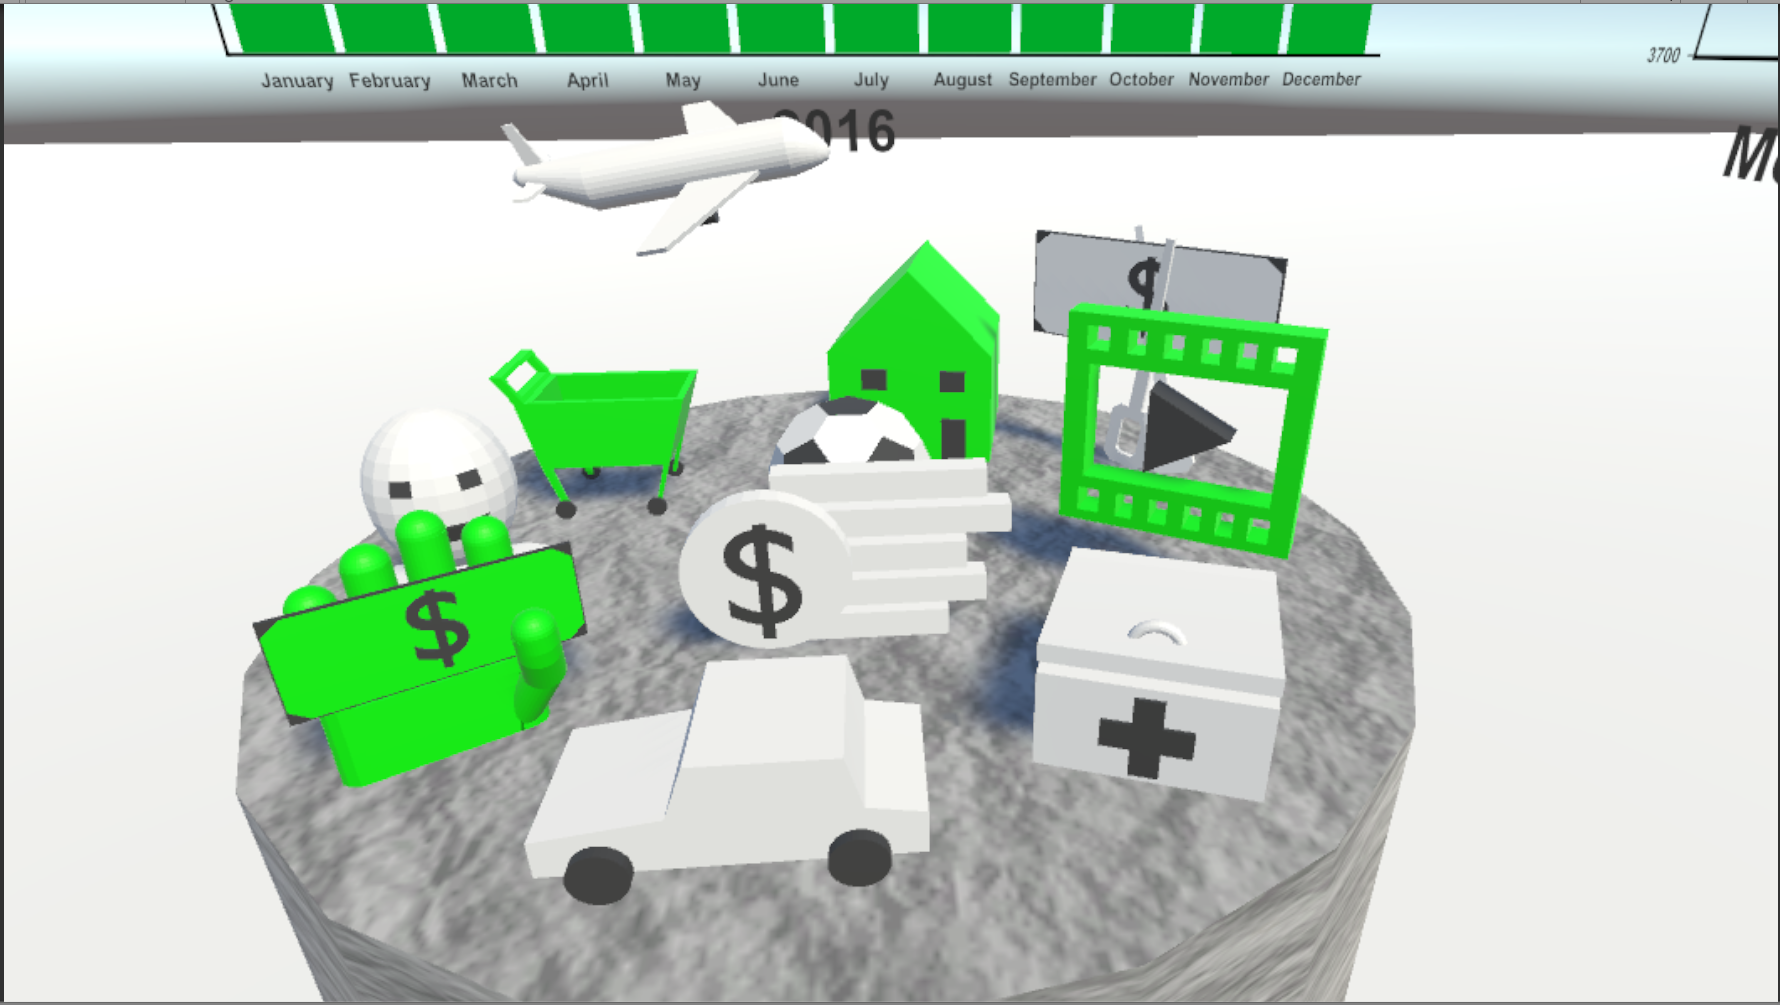
\includegraphics[width=2.35cm]{03_Figures/08_Development/View4_CategoriesFiltering.png}
		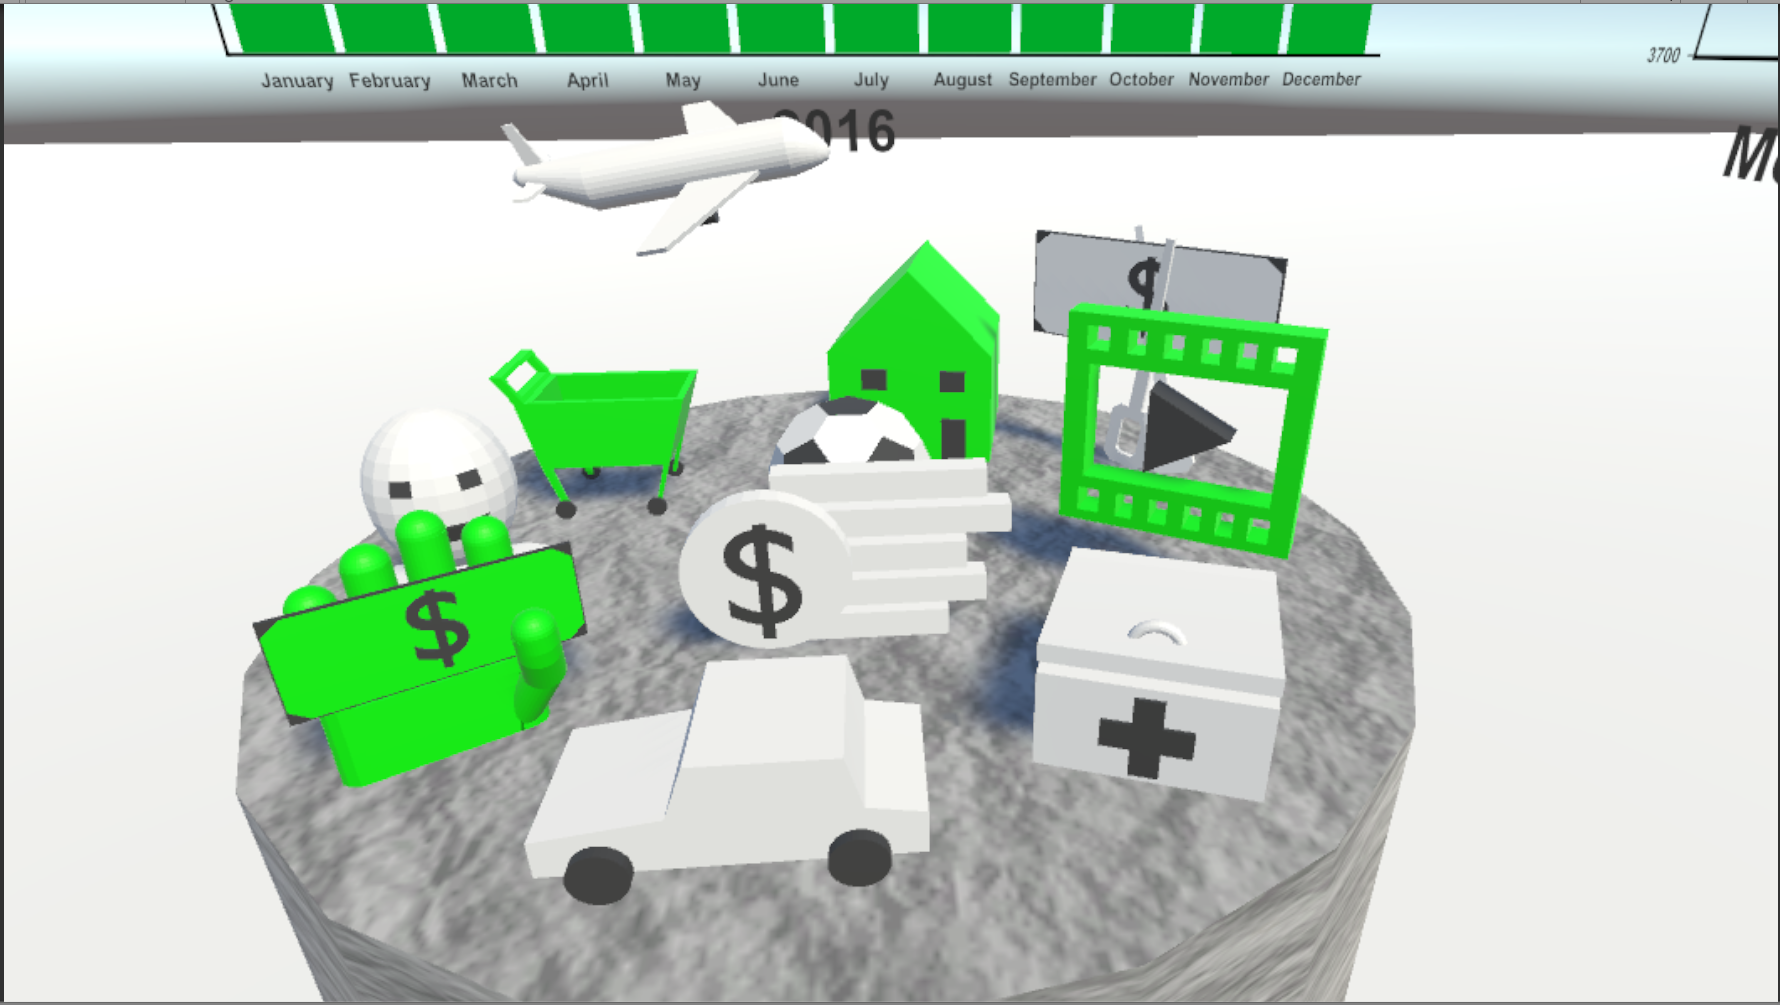
\includegraphics[width=2.35cm]{03_Figures/08_Development/View4_CategoriesFiltering.png}
		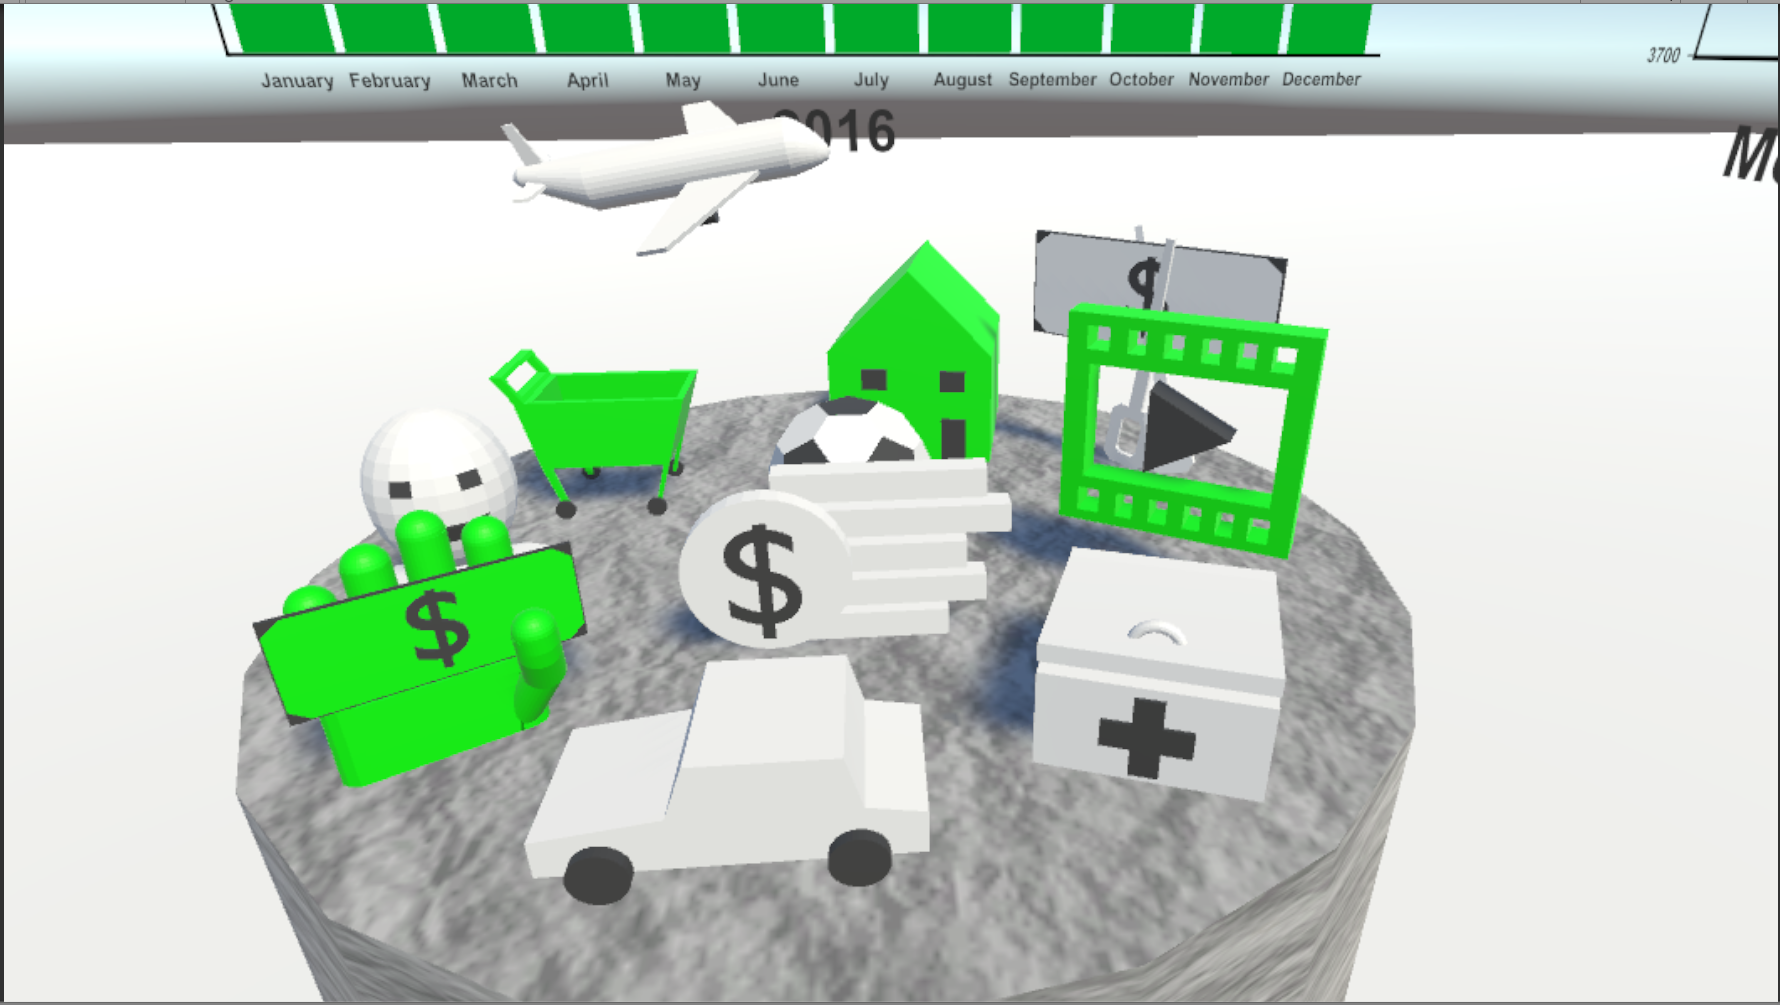
\includegraphics[width=2.35cm]{03_Figures/08_Development/View4_CategoriesFiltering.png}
		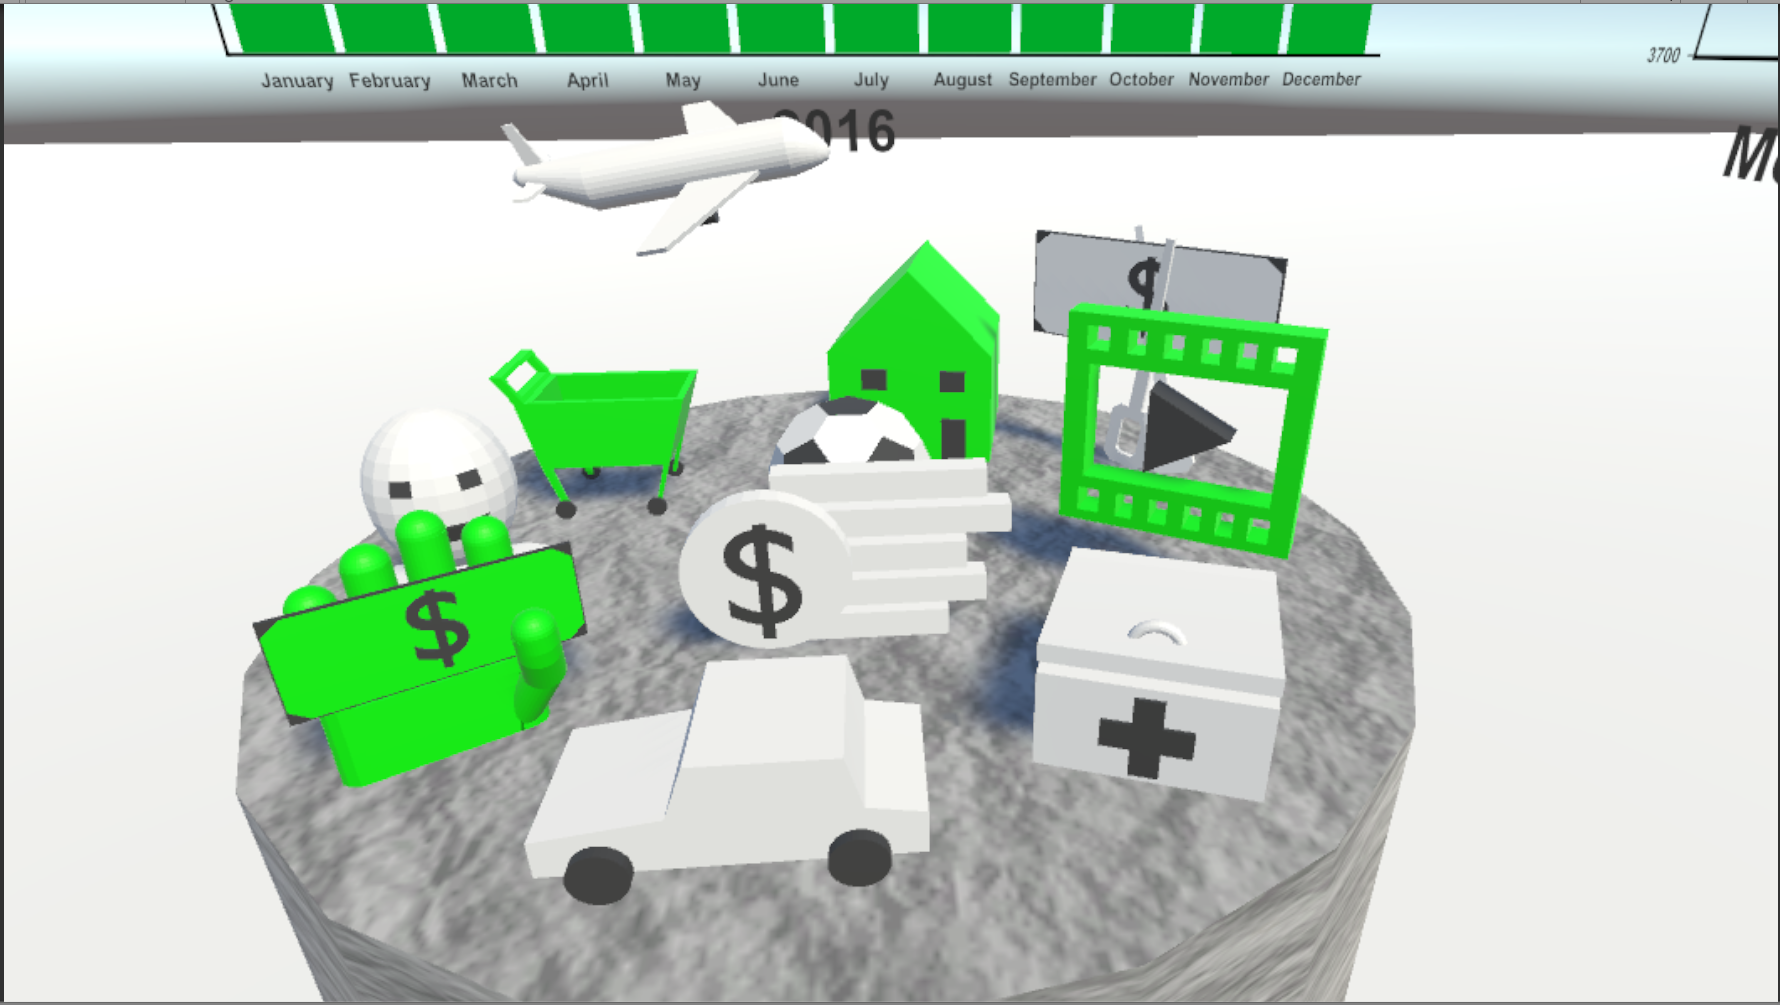
\includegraphics[width=2.35cm]{03_Figures/08_Development/View4_CategoriesFiltering.png}
		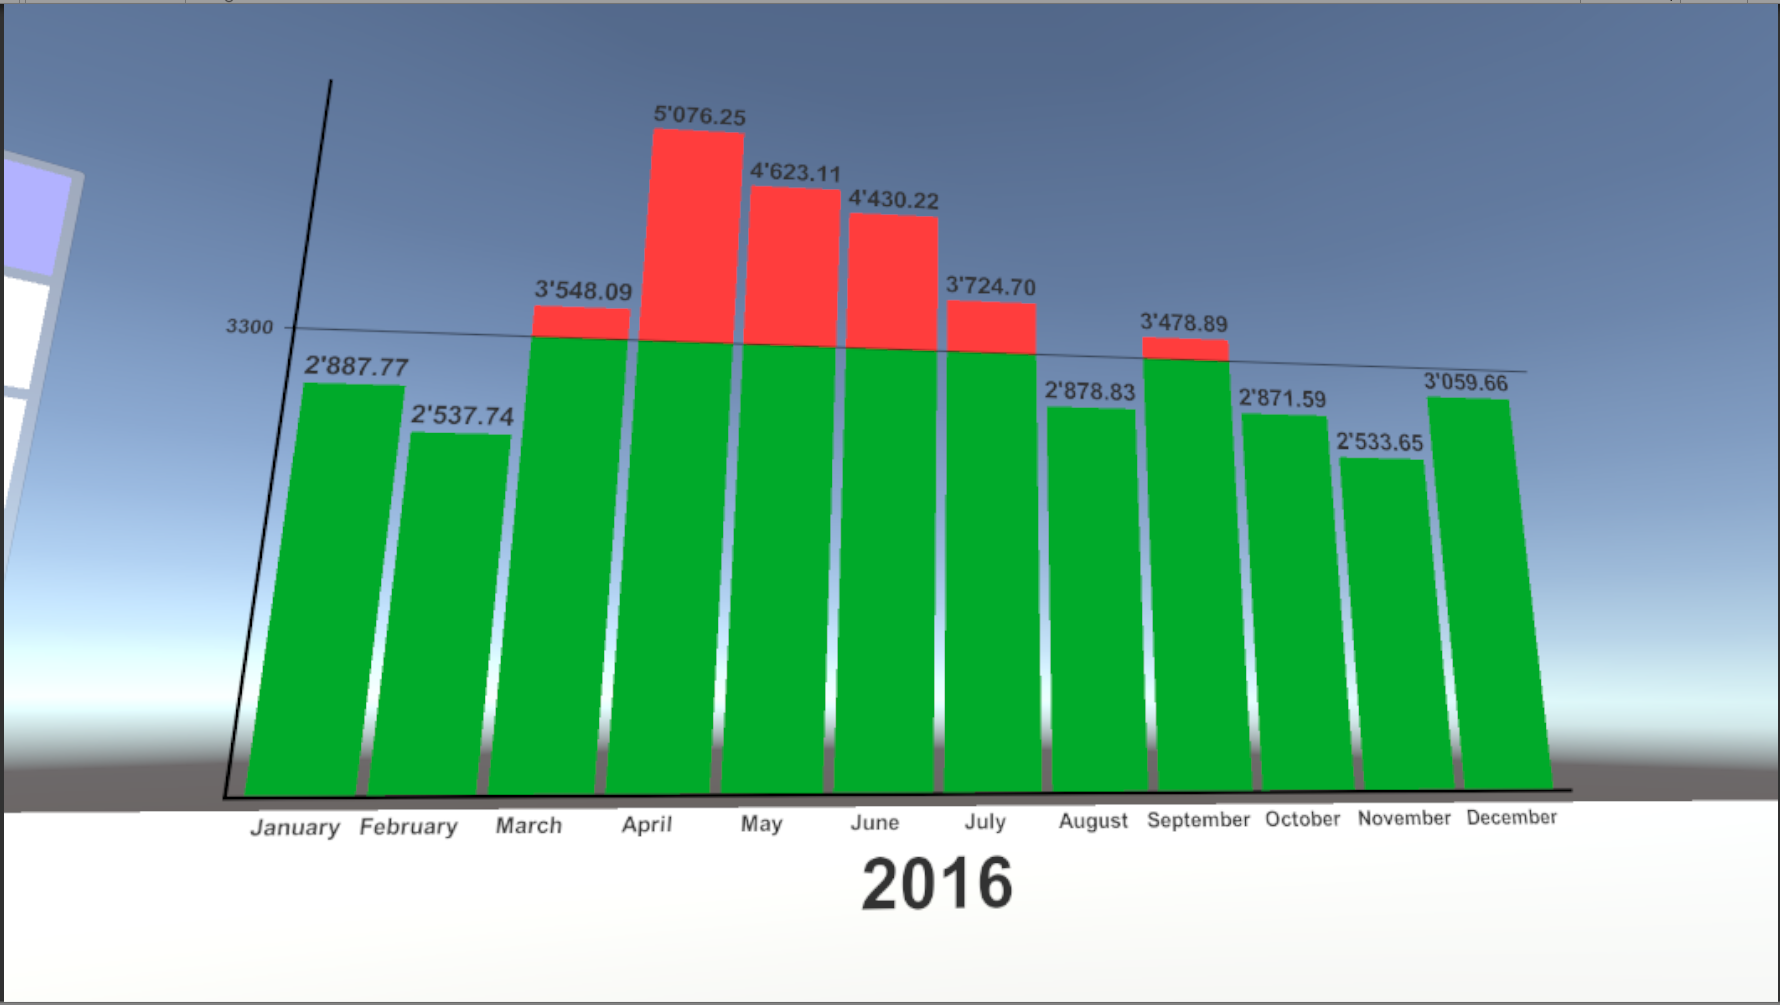
\includegraphics[width=2.35cm]{03_Figures/08_Development/View1_YearOverview.png}
		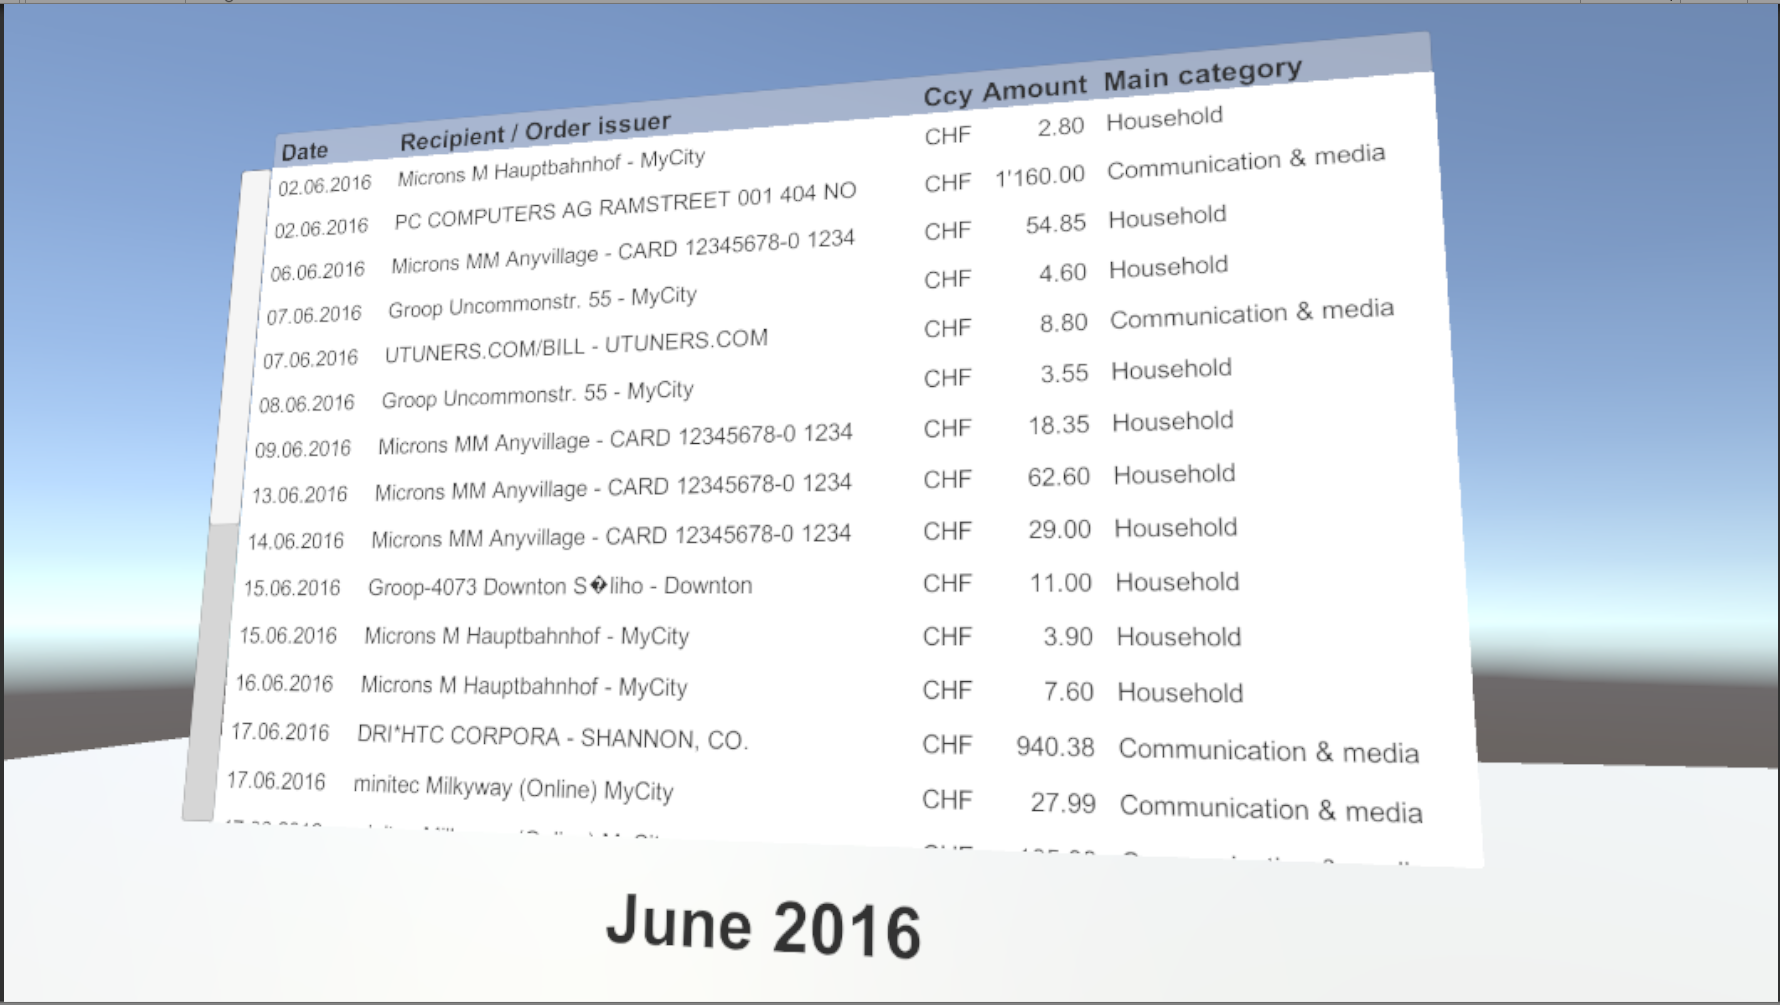
\includegraphics[width=2.35cm]{03_Figures/08_Development/View5_FinTransactionsOverview.png}
		\caption{Visualized flow of views in prototype for Scenario 4}
		\label{fig:scenariofourprototype}
	\end{center}
\end{figure}

\textbf{Evaluation:} The most interaction steps are spent on activating all relevant categories. Once the current month has been selected in the Year Overview, the Month Overview shows a cumulative chart with all expenses that can give an indication if and by when the threshold line might be reached if not already exceeded. For more details, the Transactions Overview table can be consulted on the right side to see what transaction had already been executed on the account. The exclusivity is also high since the categories can be individually toggled and the month selection is also don exclusively. For the comprehensibility, again some interpretation is required in order to understand how much budget is left until the end of the month.
\begin{itemize}[noitemsep,nolistsep]
	\item Min. number of steps: \textbf{5 - 6}
	\item Exclusivity: \textbf{High}
	\item Comprehensibility: \textbf{Medium}
\end{itemize}


%-----------------------------------
%	SUBSUBSECTION 1
%-----------------------------------

\subsubsection{Conclusion: Scenario 3}

For scenario 4, the summary of both evaluations are shown in Table \ref{tbl:scenariofourcomparison}. Compared to scenario 3, the e-banking cannot rely on the account-specific view anymore for this scenario and has to rely on the "Expenses" page again. With this flow, the prototype beats the e-banking both in the minimum number of steps required as well as in the comprehensibility die to its inherent design for such scenario questions. In terms of the exclusivity, both applications apply the same filters and therefore have the same exclusivity at the end.
\begin{table}[h]
	\begin{center}
		\begin{tabular}{ | p{3.2cm} | p{3.8cm} | p{3.5cm} | p{2.5cm} | }
			\hline
			\textbf{Metric} & \textbf{E-Banking} & \textbf{Prototype} & \textbf{Winner} \\
			\hline
			Min. no. of steps: & 12 & 5 - 6 & Prototype \\
			\hline
			Exclusivity: & High & High & Draw \\
			\hline
			Comprehensibility: & Low & Medium & Prototype \\
			\hline
		\end{tabular}
		\caption{Scenario 4: Comparison of prototype and e-banking}
		\label{tbl:scenariofourcomparison}
	\end{center}
\end{table}


%----------------------------------------------------------------------------------------
%	SECTION 2
%----------------------------------------------------------------------------------------

\section{Conclusion}

A summary of the conclusions of all individual scenarios together with the corresponding winner is shown in Table \ref{tbl:scenariosummary}. It can be seen that regarding the minimum amount of steps required, the prototype in most cases has to upper hand or at least is equally efficient as the e-banking. This shows that with the prototype it generally is simpler and faster to reach the point where an open question in a specific scenario can be answered. With the multiple different views that are all linked together, additional benefits can be created the more navigation is required compared to the traditional e-banking solution. In terms of exclusivity, generally the e-banking provides more direct answers which is also related to the fact that compared to the prototype many more different filters can be applied compared to the prototype which only has two was of filtering. As for the comprehensibility, on average both solutions are more or less equal. When information about a specific account in the last 30 days is required, the e-banking is hard to beat by the prototype application, but as soon as the queries become more complex and have to cover a longer period of time, the benefits of the prototype application can shine. \newline
Overall it can be said that in the scenario testing, the prototype application has proven its worthiness and that it can compete with the traditional solution. With further research into the prototype and more advanced filtering possibilities, the prototype has good chances to surpass the effectiveness of e-banking.
\begin{table}[h]
	\begin{center}
		\begin{tabular}{ | p{3.2cm} | p{2.5cm} | p{2.5cm} | p{2.5cm} | p{2.5cm} | }
			\hline
			\textbf{Metric} & \textbf{Scenario 1} & \textbf{Scenario 2} & \textbf{Scenario 3} & \textbf{Scenario 4} \\
			\hline
			Min. no. of steps: & Prototype & Prototype & Draw & Prototype \\
			\hline
			Exclusivity: & E-Banking & Draw & E-Banking & Draw \\
			\hline
			Comprehensibility: & Draw & Draw & E-Banking & Prototype \\
			\hline
		\end{tabular}
		\caption{Scenarios: Summary of comparison between prototype and e-banking}
		\label{tbl:scenariosummary}
	\end{center}
\end{table} \newline

